
\chapter{Machine Learning Application: Force Seeking System}\label{chapter:ftml}

	
\chapterintro*
Wireless communications plays an essential role in the vision of future cyber-physical systems (CPS) which includes having more sensors and actuators, and, hence, more information transferred wirelessly. Many system and environmental features of industrial CPS affect the success of wireless communications on the factory floor. In this article, the author considers a representative industrial CPS use case of a robot arm control system equipped with a force-torque sensor. Movement of the arm is controlled by a robot controller applying a downward pressure on a spring assembly until a predetermined force is detected. This movement of the robot arm is tracked by a vision-based ground truth measurement system. This remote observer provides readings about the position of the robot arm where these readings are used to estimate the signal-to-interference ratio of the wireless link. By using readings from the remote observer, an estimation system is developed using machine learning regression techniques.  This work demonstrates the practicality of combining statistical analysis with machine learning to indirectly estimate signal-to-interference of the wireless communication link using measurements from the remote observer.  Results from the statistical analysis and the performance of the machine learning system are presented.  A supervised machine learning (ML) approach is used for the wireless channel quality estimation. the impact of selected system features on the estimation performance of various ML algorithms and compare their performance is studied.  Moreover, the author investigates the impact of the training and the estimation period on the performance of the proposed approach. The results provide insights about the impact of wireless communications on cyber-physical systems and an example of employing machine learning to improve industrial wireless deployments. 


	
	\section{Introduction} \label{ftml:sec:intro}    
	Industrial wireless systems (IWSs) are being deployed in various industrial environments due to the advances of wireless protocols and devices for cyber-physical systems (CPSs). Application domains for IWSs include flexible manufacturing, safety, process control, alerting and monitoring\cite{Candell2018.IWSGuide}. The advantages of deploying wireless communications in industrial applications due to the absence of cabling include ease of scale, flexibility, and lower cost compared the wired counterpart. Nevertheless, there are challenges in wireless deployments~\cite{Sisinni2018,Bello2017,Pang2017.WirelessChallenges}. The main cause of these challenges is the unpredictable and random nature of wireless channels. Challenges include latency uncertainty, error uncertainty, and  increased information loss when operating in the presence of significant interference and limited spectral resources~\cite{Candell2017.SAS.IWSWorkshopReport}. In addition, the quality of wireless data communications is impacted by various wireless channel impairments such as path loss, fading, multi-path, and interference. As a result, a careful design of wireless communications and control networks is required to deal with these impairments~\cite{Lu2016.WirelessCPS,Kim2017.WirelessCodesign}.    
    
    One of the major challenges in designing IWSs and the underlying industrial systems is interference detection and mitigation. Interference can result from various narrow-band or wide-band sources including  coexisting wireless systems, intentional jamming sources, and non-communications intended devices such as industrial equipment and microwave ovens~\cite{Chiwewe2015.Survey.CR.Intf}. Interference can degrade the communication quality of service (QoS) significantly and hence IWS designers consider various interference management techniques.   

    In~\cite{Candell_ISIT_2019}, the authors presented a method that deploys random forest regression to estimate the signal to interference ratio (SIR) of the communication channel within a robotic arm force-seeking scenario in which the force value signal is transmitted over a wireless local area network (WLAN)~\cite{IEEE802.11ac}. In that work, the authors have presented the testbed setup, the statistical relations between various measured features, and the performance of the proposed machine learning random forest algorithm as in~\cite{Candell_ISIT_2019}.  
    
    In this work, the same testbed setup is deployed to explore, in more detail, the impact of machine learning on the performance of the detection algorithm.  It is also endeavored to understand the impact of various features in the training data set. Hence, position data is used from a vision-based tracking system, a distant observer, to train a channel quality estimator to infer the SIR experienced by both the wireless access point and the wireless station used within the experiment. Five different features are extracted from the position data captured by the vision system. The contributions of this paper are summarized as follows:
    \begin{itemize}
        \item The work briefly explains the proposed algorithm for SIR estimation, the testbed setup, and the features extracted from the position data.
        \item Various machine learning regression schemes are compared for SIR estimation, thereby demonstrating the superior performance of various ensemble-based approaches.
        \item Impact of individual features are studied regarding the performance of the proposed algorithm to understand the correlation between the interference level to each of these features. Hence, the correlation between physical systems behavior and the underlying quality of the wireless communications channel is better understood. 
        \item Finally, an analysis on the impacts of measurement interval and the training set size on the performance of the ML algorithms is provided.
    \end{itemize}
    
%\section{Related Work}    
%In the literature, two types of interference signals are considered, namely, intentional or unintentional interference. Methods to estimate, avoid, or mitigate interference are required for the deployment of reliable and deterministic IWSs. Machine learning has been widely used to detect and estimate interference information to enhance the performance of interference managment algorithms.  
% 
% The interference analysis in cyber-physical systems (CPSs) has been considered in multiple works for various scenarios. In~\cite{8639006}, in-network interference mitigation techniques are discussed for ultra reliable low-latency wireless communications systems. The paper focused on mutual interference mitigation in an industrial automation setting, where multiple transmissions from controllers to actuators interfere with each other. In \cite{Kumar2019}, an interference mitigating receiver architecture is proposed. The application scenarios are smart homes and modern factories where dense wireless communications devices exist. Moreover, in~\cite{Bhushan2014.NetworkDesensUsingIntfCancellation}, interference cancellation of transmissions from neighboring cells in a 5G cellular network is presented. In~\cite{Gomes2017.LQEinWSNs}, a method using a dedicated node for link quality estimation (LQE)  obtained through received data packets to identify interference and multi-path without introducing additional traffic is presented. In~\cite{Baccour2012.SurveyOnLinkEstimation}, a taxonomy of channel link quality techniques is presented providing a valuable survey on LQE algorithms and asserting the importance of link quality estimation in IWSs. In~\cite{Frounhoffer.Troubleshooting}, failure analysis and wireless network troubleshooting are performed whenever the CPS is not functioning properly. Interference analysis is one major part of the troubleshooting procedure which is performed through traffic patterns and wireless spectrum analysis. Also, in~\cite{NIST.InterfCoexCritical}, the use of spectrum analysis for interference detection and estimation is proposed for IWSs. 
% 
%On the other hand, intended interference (i.e., jamming) can lead to service denial or poor performance in wireless networks. In~\cite{8631535}, a literature review was presented which includes an overview of recent research efforts on networked control systems under denial-of-service attacks such as jamming attacks in wireless channels. One of the discussed challenges is how to achieve ultra-reliable low-latency "signalling" within industrial applications. In~\cite{Cetinkaya_2019}, a discussion is also provided on the recent developments concerning the design of attack-resilient control and communication protocols. Generally, a jamming attacker can block transmission of packets by emitting strong interference signals to a wireless channel \cite{1637931,5473884}. Jamming attacks can target various wireless technologies and hence can become a major concern for control systems, since they are easy to launch \cite{5473884}. It was shown in \cite{10.1007/978-3-319-07788-8_40} that off-the-shelf hardware can be used for generating jamming attacks on wireless networks. In cases of physical-layer attacks, the jamming attacker targets a frequency band and is not required to follow the wireless protocol where it can cause a decrease in the SIR thus preventing the receiver from successfully detecting transmitted packets \cite{10.1007/978-3-319-07788-8_40}. In the case of MAC-layer attacks, both the packet sender and the jamming attacker operate on the same channel; the jamming attacker’s goal is to cause packet collisions.
%In~\cite{8726803}, the authors evaluated the CPSs resilience to jamming attacks that disrupt wireless communications. They considered three jamming strategies which are the constant, random, and protocol-aware jamming. They showed through experimental results that various CPS control schemes are susceptible to constant and random jamming while the time-triggered control schemes are susceptible to protocol-aware jamming. Moreover, resilience of CPSs is also considered in~\cite{6425868,DEPERSIS2014134,7402971,7575630} where periodic jamming is considered in \cite{6425868} while the jamming strategy in~\cite{DEPERSIS2014134,7402971,7575630} is neither known nor pre-fixed. 
% 
%Machine learning has been used for detection and estimation of jamming attacks. In~\cite{Chen2019}, an unsupervised machine learning algorithm based on a multi-layer autoencoder is used to extract the interference source spectrum features. These features are then used to distinguish interference sources type and location without labeling measured data. In~\cite{7911887},  an unsupervised approach using a recurrent neural network to detect anomalies in the CPS performance and identify attacked sensors. In~\cite{Junejo2016DataDP}, a behavior based machine learning intrusion detection approach  is proposed to detect attacks at the physical process layer. The results are validated through experimental study of a real modern water treatment facility. In~\cite{Beaver:2013:EML:2584691.2584722}, the viability of machine learning methods in detecting the new threat scenarios of command and data injection is assessed. In that work, command and control communications in a critical infrastructure setting are monitored and vetted against examples of benign and malicious command traffic to identify potential attack events. In~\cite{6900095}, the authors assessed discriminating types of power system disturbances through machine learning by detecting jamming attacks. They evaluated various machine learning methods as disturbance discriminators and discuss the practical implications for deploying machine learning systems as an enhancement to existing power system architectures.
%
%Therefore, in the literature, it was shown that LQE is one important but insufficient aspect of assessing the impact of link quality on a CPS. We assert that by jointly observing the performance of the physical and wireless components of a CPS,the complete perspective of the quality of the wireless link and its impact on physical performance can be obtained. Since interference is such an important topic in the wireless CPS, we are motivated to propose a method that simultaneously (1) makes observations of the physical system using ground truth measurements, and (2) infers the quality of the wireless communication system in terms of SIR using an experimental model of a relevant use case found in industry.
    
\section{Robot Arm Force-Seeking Application}\label{sec:ftseekerapp}

\subsection{General Construction and Operation}

\begin{figure}[!tbp]
	\centering
	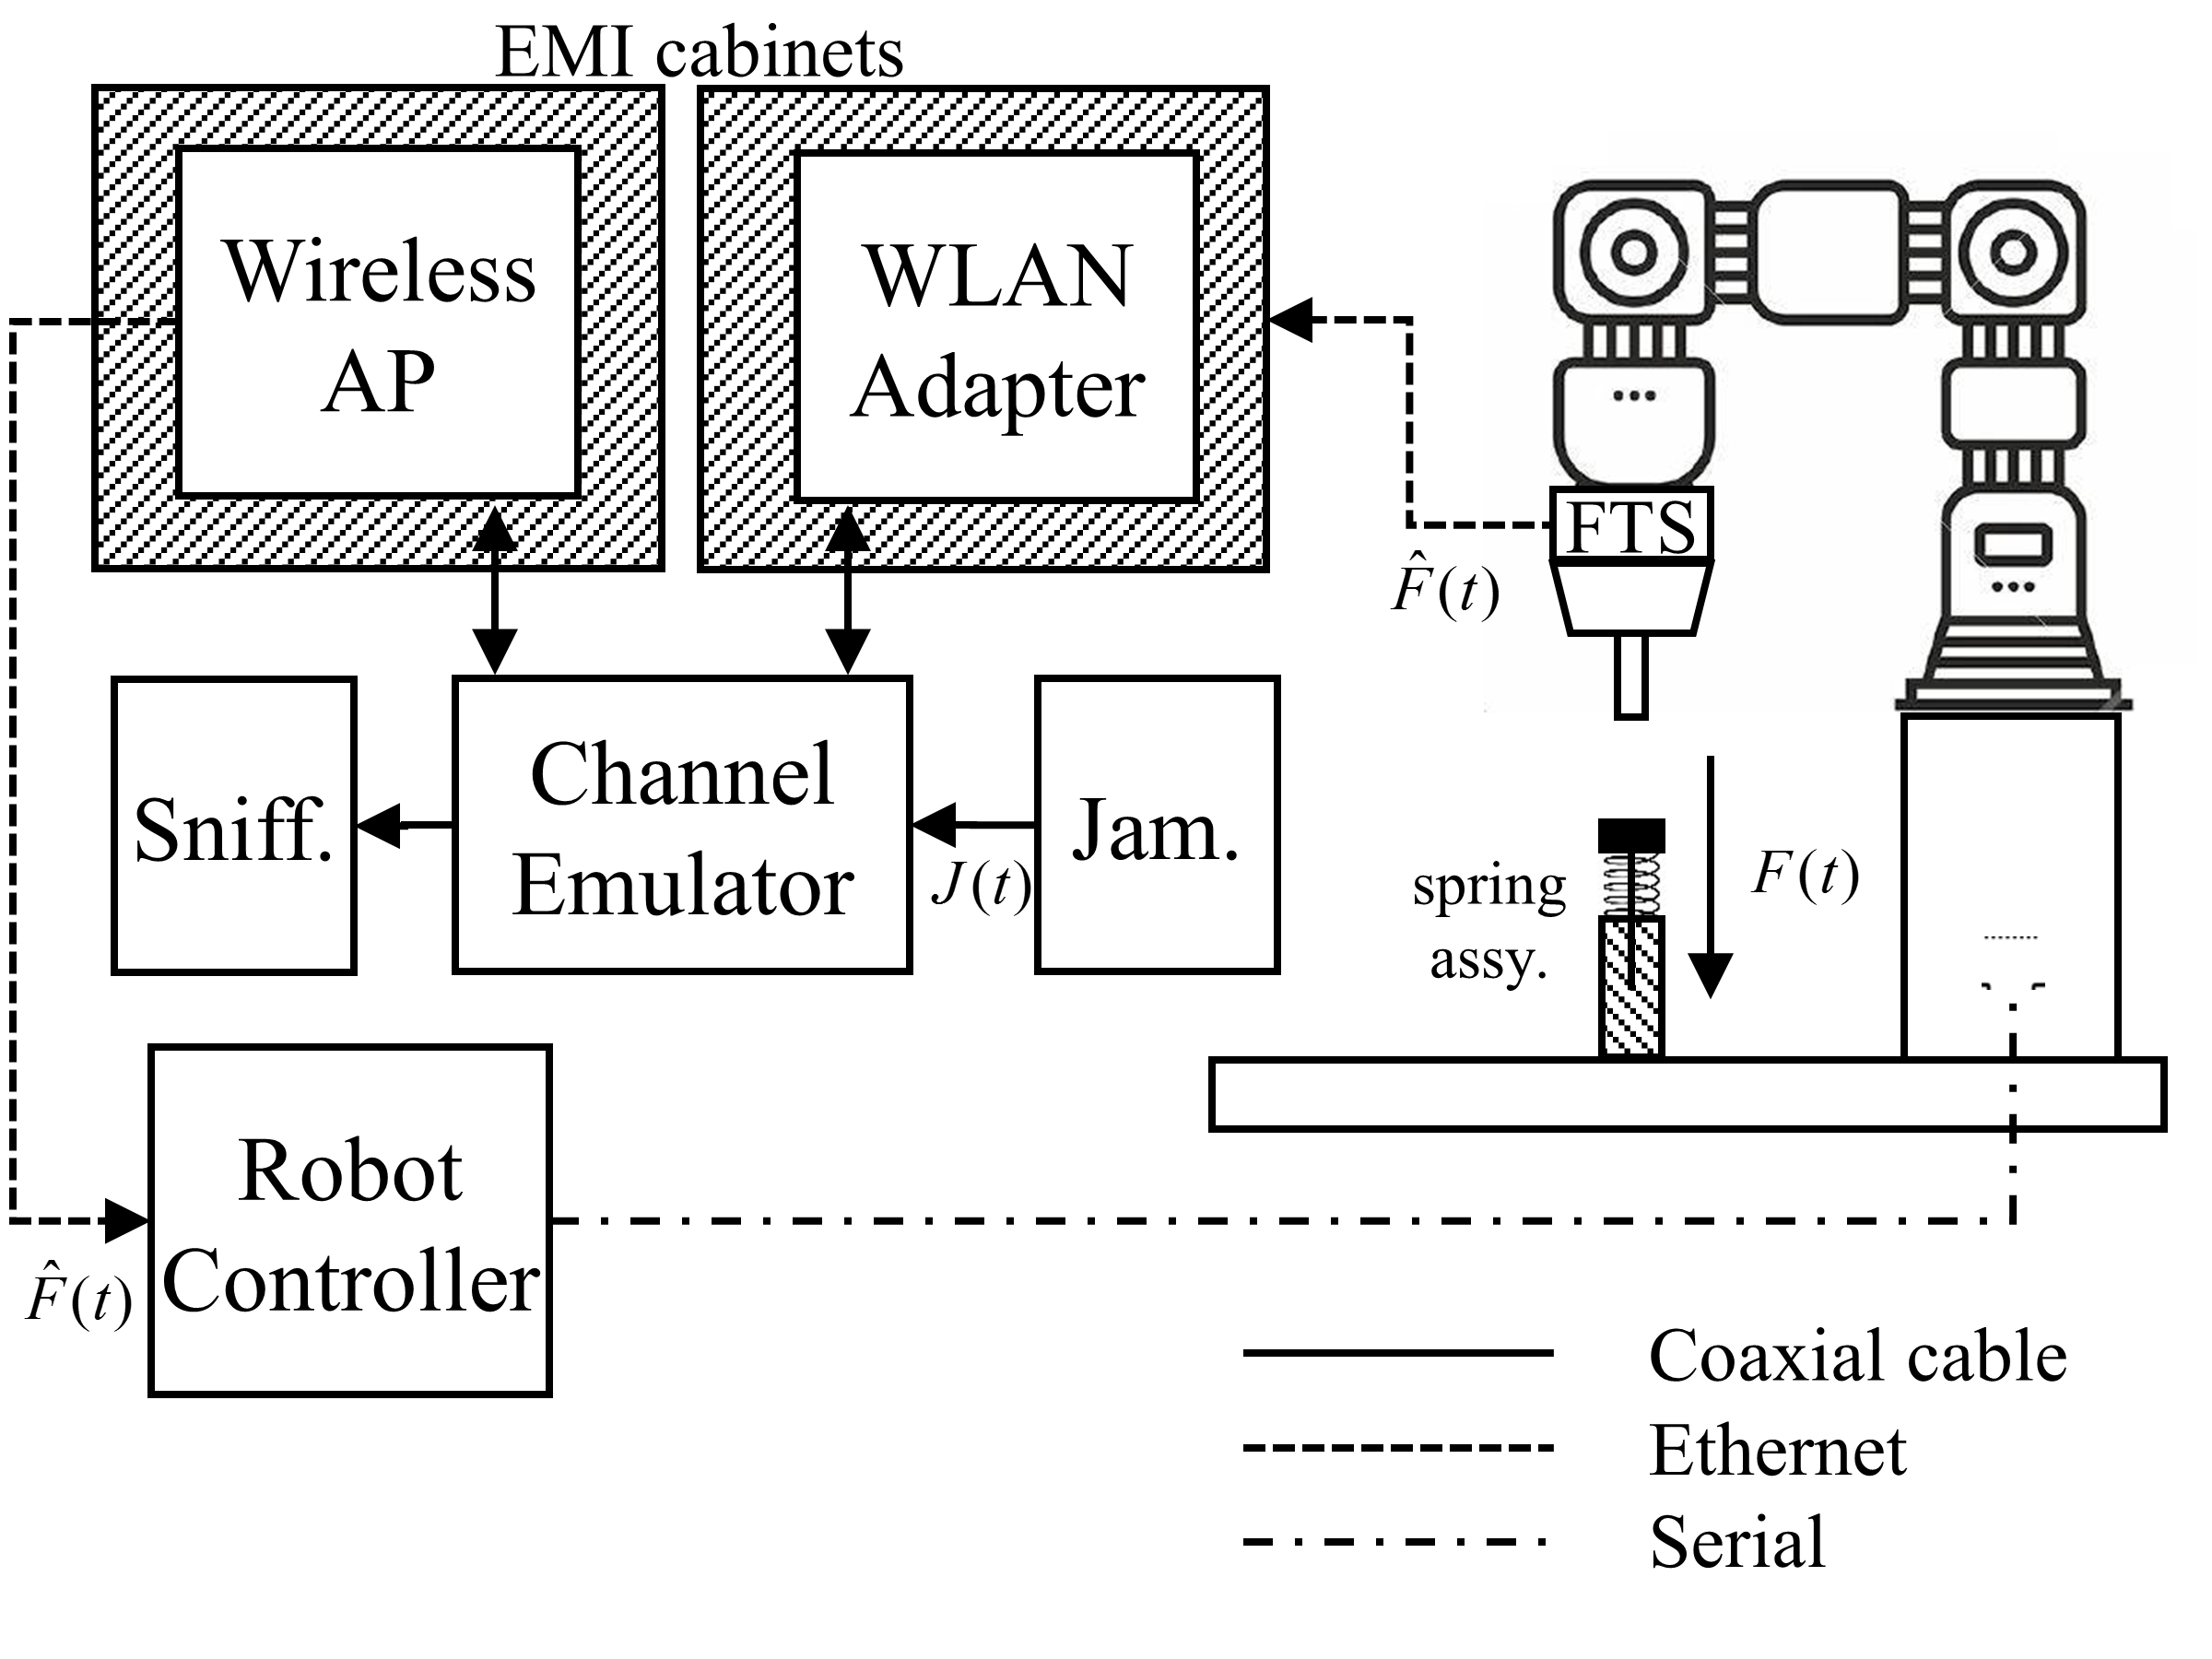
\includegraphics[width=0.65\columnwidth]{./chapter-ftml/diagrams/robotsetup}
	\caption{Robot force-seeking spring system with controlled wireless channel emulation and interference injection.}
	\label{fig:robotsetup}
\end{figure}

\begin{figure}[!tbp]
	\centering
	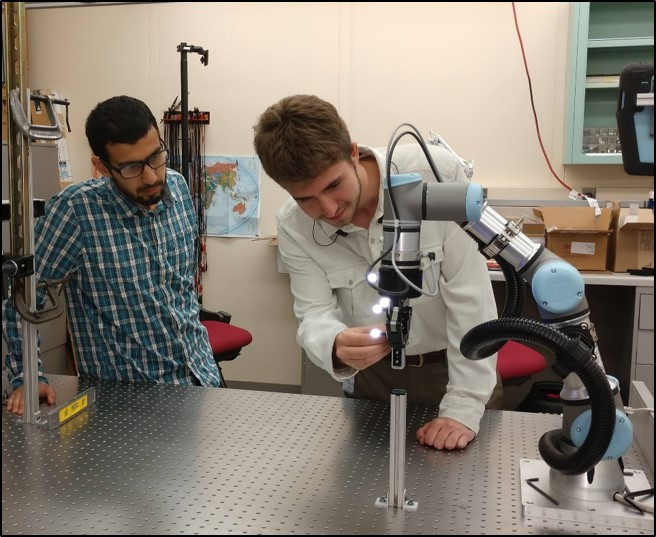
\includegraphics[width=0.65\columnwidth]{./chapter-ftml/images/PlungerExperiment}
	\caption{A photograph of the robot force-seeking experiment shows the robotic arm, the spring-based plunger, and the visual markers used for position tracking.}
	\label{fig:photo-forceseeker}
\end{figure}	

A robotic force-seeking apparatus is constructed using a Universal Robots UR-3 collaborative robot.  As illustrated in Fig.~\ref{fig:robotsetup}, the robot is fitted with a six degrees-of-freedom (DOF) force-torque sensor (FTS) followed by a probe.  The robot is programmed to apply a downward force, $F(t)$, in the $z$ direction until a force exceeding a threshold, $F_t$, is reported to the controller.  The robot encounters the force threshold through a fixed plunger-spring assembly.  The force in the spring is governed by the equation $F(t)=kl$ where $k$ is the spring constant and $l$ is the spring deflection.  The robot will push the spring downward repeatedly for the duration of 30 minutes.  Plunger movement is limited by a hard stop which will reset the height of the robot arm.  A photograph of the force-seeking apparatus is shown in Fig.~\ref{fig:photo-forceseeker}.  The illuminated spheres shown in the photo are infrared markers used by the remote observer to track the position of the probe.

\subsection{Components}

Referring again to Fig.~\ref{fig:robotsetup}, the system is composed of the following components:

\begin{description}
	\item[Robot] The robotic arm applies a downward force along the z-axis to the plunger-spring assembly.  The robot is a 6-DOF rigid body manipulator in which all joints have a full 360 degrees of motion.  For the experiment, the robot is configured such that it would replicate the action of a robot applying a force to push a small part into place within an automotive assembly work-cell~\cite{Cossio2012.RoboticsHandbook}.  The robot is mounted on a motionless optics table in which mechanical vibration is dampened.
	
	\item[Robot Controller] The robot controller (RC) provides the motion control function of all joints on the robot.  The RC is responsible for controlling motion while searching for a force feedback signal.
	
	\item[Force Torque Sensor] The force torque sensor (FTS) provides continuous force and torque readings at a rate of 125 Hz.  Readings from the FTS include force measurements in Newtons along the three Cartesian axes, $x$, $y$, and $z$, and three torque readings in Newton-meters (N-m) about each axis.  The FTS is designed to communicate with the RC through an Ethernet connection. 
	
	\item[Robot End-effector] The robot end-effector (REEF) is a rigid body probe attached to the end of the robot arm just after the FTS.  The REEF is used to make contact with the plunger-spring assembly.   
	
	\item[Wireless Components]  The wireless Ethernet adapter (WEA) replaces the Ethernet connection between the FTS and the RC with a Wi-Fi connection.  The adapter supports the IEEE 802.11 b, g, n, and ac modes. The WEA connects to the RC through a wireless access point (WAP).
	
	\item[Jammer] The jammer provides the source of interference, $J$, which is directly injected into the wireless channel.  For simplicity, interference is injected as non-modulated additive white Gaussian noise (AWGN).  The power of $J$ at each receiver is determined by its distance to the jammer.
	
	\item[Channel Emulator] The channel emulator (CE) provides the capability to control the electromagnetic channel between the WEA and the WAP.  The CE supports frequencies between 1 GHz and 6 Ghz and has an instant bandwidth of 250 MHz. It also supports a channel impulse response of 13 taps with a minimum time resolution of 4 ns making the replication of close-quarter multi-path reflections possible.  As shown in Fig.~\ref{fig:robotsetup}, all wireless devices are connected to the CE.
	
	\item[Electromagnetic Interference Cabinets] The electromagnetic interference (EMI) cabinets provide isolation between devices such that communication between devices does not occur through radiated leakage.
	
	\item[Wireless Sniffer]  A wireless sniffer (WS) is used to monitor wireless traffic during operation. The sniffer is connected to a laptop computer running Wireshark, and packet logs are used for offline analysis of network events.
	
	\item[Vision Tracking System]  An OptiTrack VS120 Trio is used as the vision-based tracking system (VTS) to produce accurate ground truth measurements of the probe position.  Position estimates along the $z$-axis are captured at the maximum video frame rate of 120 frames per second.  Each estimate includes time and position.
	
\end{description}

\subsection{Robot Arm Motion Control}

\begin{figure}[tbp]
	\centering
	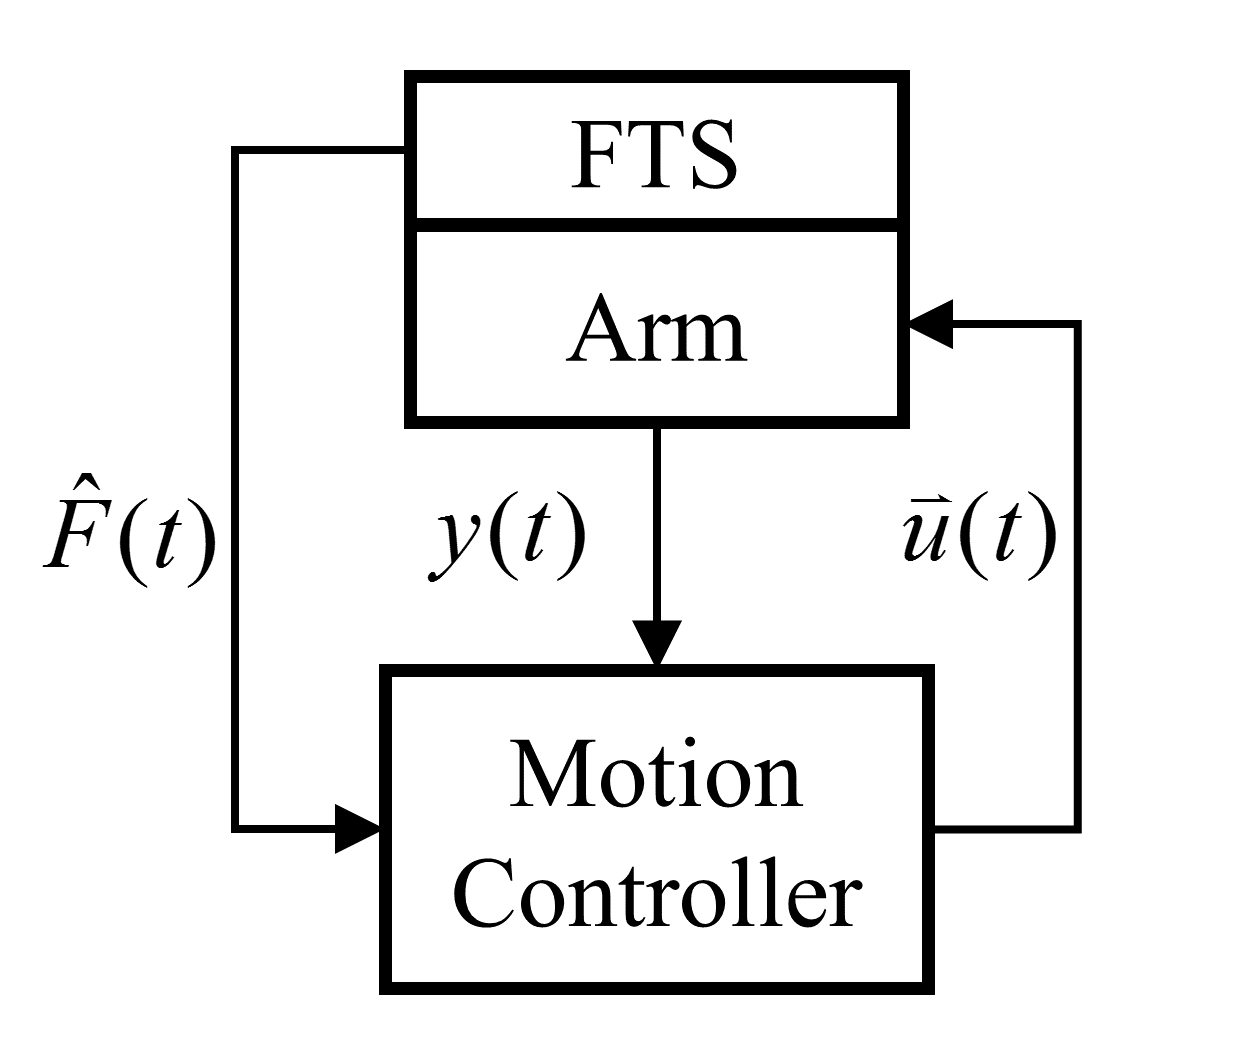
\includegraphics[width=0.4\columnwidth]{./chapter-ftml/diagrams/reef-model}
	\caption{Feedback signal flow model of the force-seeking controller}
	\label{fig:reefmodel}
\end{figure}

A diagram of the control system for the robotic manipulator is shown in Fig.~\ref{fig:reefmodel}.  The UR-3 is constructed of the manipulator assembly and the RC assembly.  The internal construction of the robot arm is irrelevant for this experiment, but it is assumed that the arm produces encoder positions $y(t)$ for each joint.  It is also assumed that the robot arm accepts actuation signals $\vec{u}(t)$ from the motor drives located in the RC.  Both $y(t)$ and $\vec{u}(t)$ are conveyed through wired connections. The force sensor signal $\hat{F}(t)$ is produced by the FTS and is conveyed via an IEEE 802.11 wireless connection. The RC is programmed to move a probe connected to the end of the manipulator downward along a linear path until a force of at least 5 N is detected.  The RC will not move the arm during the force-seeking operation unless it receives an FTS signal; therefore, the duration and continuity of the movement of the arm will be impacted by unreliable communication between the FTS and the RC.

\subsection{RF Emulation Scenario}\label{sec:rfemulator}

\begin{figure}[tbp]
	\centering
	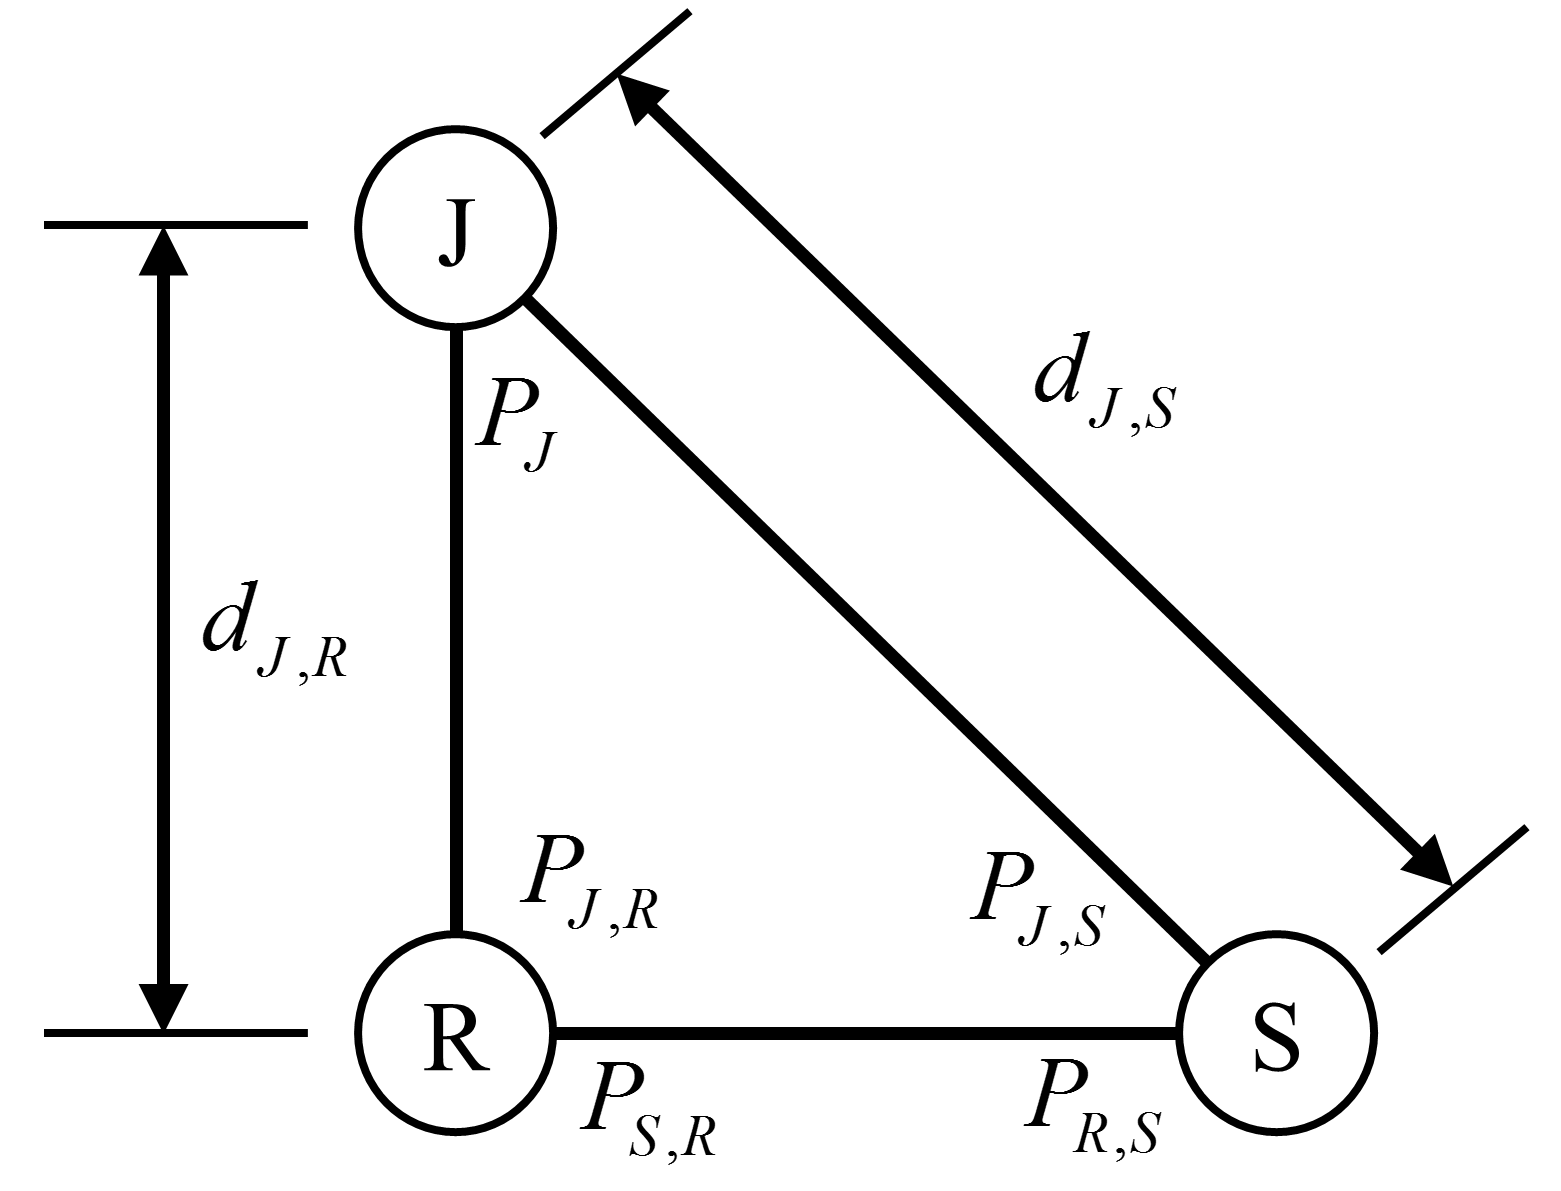
\includegraphics[width=0.5\columnwidth]{./chapter-ftml/diagrams/emulation-model}
	\caption{RF emulation scenario design of the robotic force-seeking scenario.}
	\label{fig:rf-emulation-scenario}
\end{figure}

The CE is programmed using a graphical user interface in which the wireless scenario is modeled.  Scenarios are composed of radios, platforms, and links.  Platforms represent the physical machine on which a radio may be deployed.  Platforms may be mobile or stationary, ground-based or aerial. Radios are assigned to platforms, and each radio is associated to a physical port on the emulator.  Links are representations of the physical connections between radios.  Each link has an associated path loss and multi-path representation.  Path loss is implemented according to Friis equation~\cite{Shaw2013.Frii} simplified as 
$P_r = P_t + C - 10\gamma\log_{10}\left( d \right)$, 
where $P_r$ is the received power, $P_t$ is the transmitted power, $C$ is a characteristic constant representing characteristics of the channel and electronics, $\gamma$ is the path loss exponent, and $d$ is the distance between transmitter and receiver.  For simplicity, it is assumed that path loss occurs in accordance with the square of the distance ($\gamma=2$); however, in practice, the path loss exponent is usually greater, causing a more rapid loss of signal power over the same distance~\cite{Candell2017.NIST1951}.  Since the focus of this work is to infer signal quality from ground truth measurements, the path loss exponent is inconsequential to this analysis.

%\begin{equation}
%    P_r = P_t + D_t + D_r + \gamma 10\log_{10}\left( \frac{\lambda}{4 \pi d} \right)
%    \label{eq:frii}
%\end{equation}

Shown in Fig.~\ref{fig:rf-emulation-scenario} is the general scenario for the wireless communication system employed for the force feedback control system.  In the figure, there are three nodes, a wireless router (R), a wireless station (S), and a jammer (J).  The router and station transmit with nominal power that is dependent upon the 802.11 protocol. The jammer transmits with constant power, and its impact on the scenario depends on its position relative to the other nodes.  The distance between J and R is denoted by $d_{J,R}$, and the distance between the J and S is denoted by $d_{J,S}$.  The resulting signal-to-interference power ratio (SIR) for the router is defined in decibels as $SIR_{J,R} = P_{S,R}-P_{J,R}$ which is the power received by the router of the station signal divided by the power of interference experienced at the router.  Similarly, the SIR experienced at the station is defined as $SIR_{J,S} = P_{R,S}-P_{J,S}$ which is the received signal power of the router at the station divided by the interference power experienced at the station.

For each experiment, the location of the J is adjusted to produce a desired SIR.  Each time the location of J is changed, the robot is allowed to operate for a period of 30 minutes.  This included periods of inaction by the robot when the SIR prohibits movement of the arm.  The SIR setting was validated for each run using a real-time spectrum analyzer connected directly to the emulator.

	
	\section{Initial Investigations}

The contents of this section explain the approach, methodology, and results of the initial investigations using machine learning to infer the \gls{sir} of a single radio link using situational awareness information from a camera system as published in~\cite{CandellISIE2019.Conf} with data made available at https://doi.org/10.18434/m32077.
%~\cite{https://doi.org/10.18434/m32077}.

\subsection{Data Analysis}\label{ftml-conf:sec:dataanalysis}

%	\begin{figure}[tbp]
%	    \centering
%	    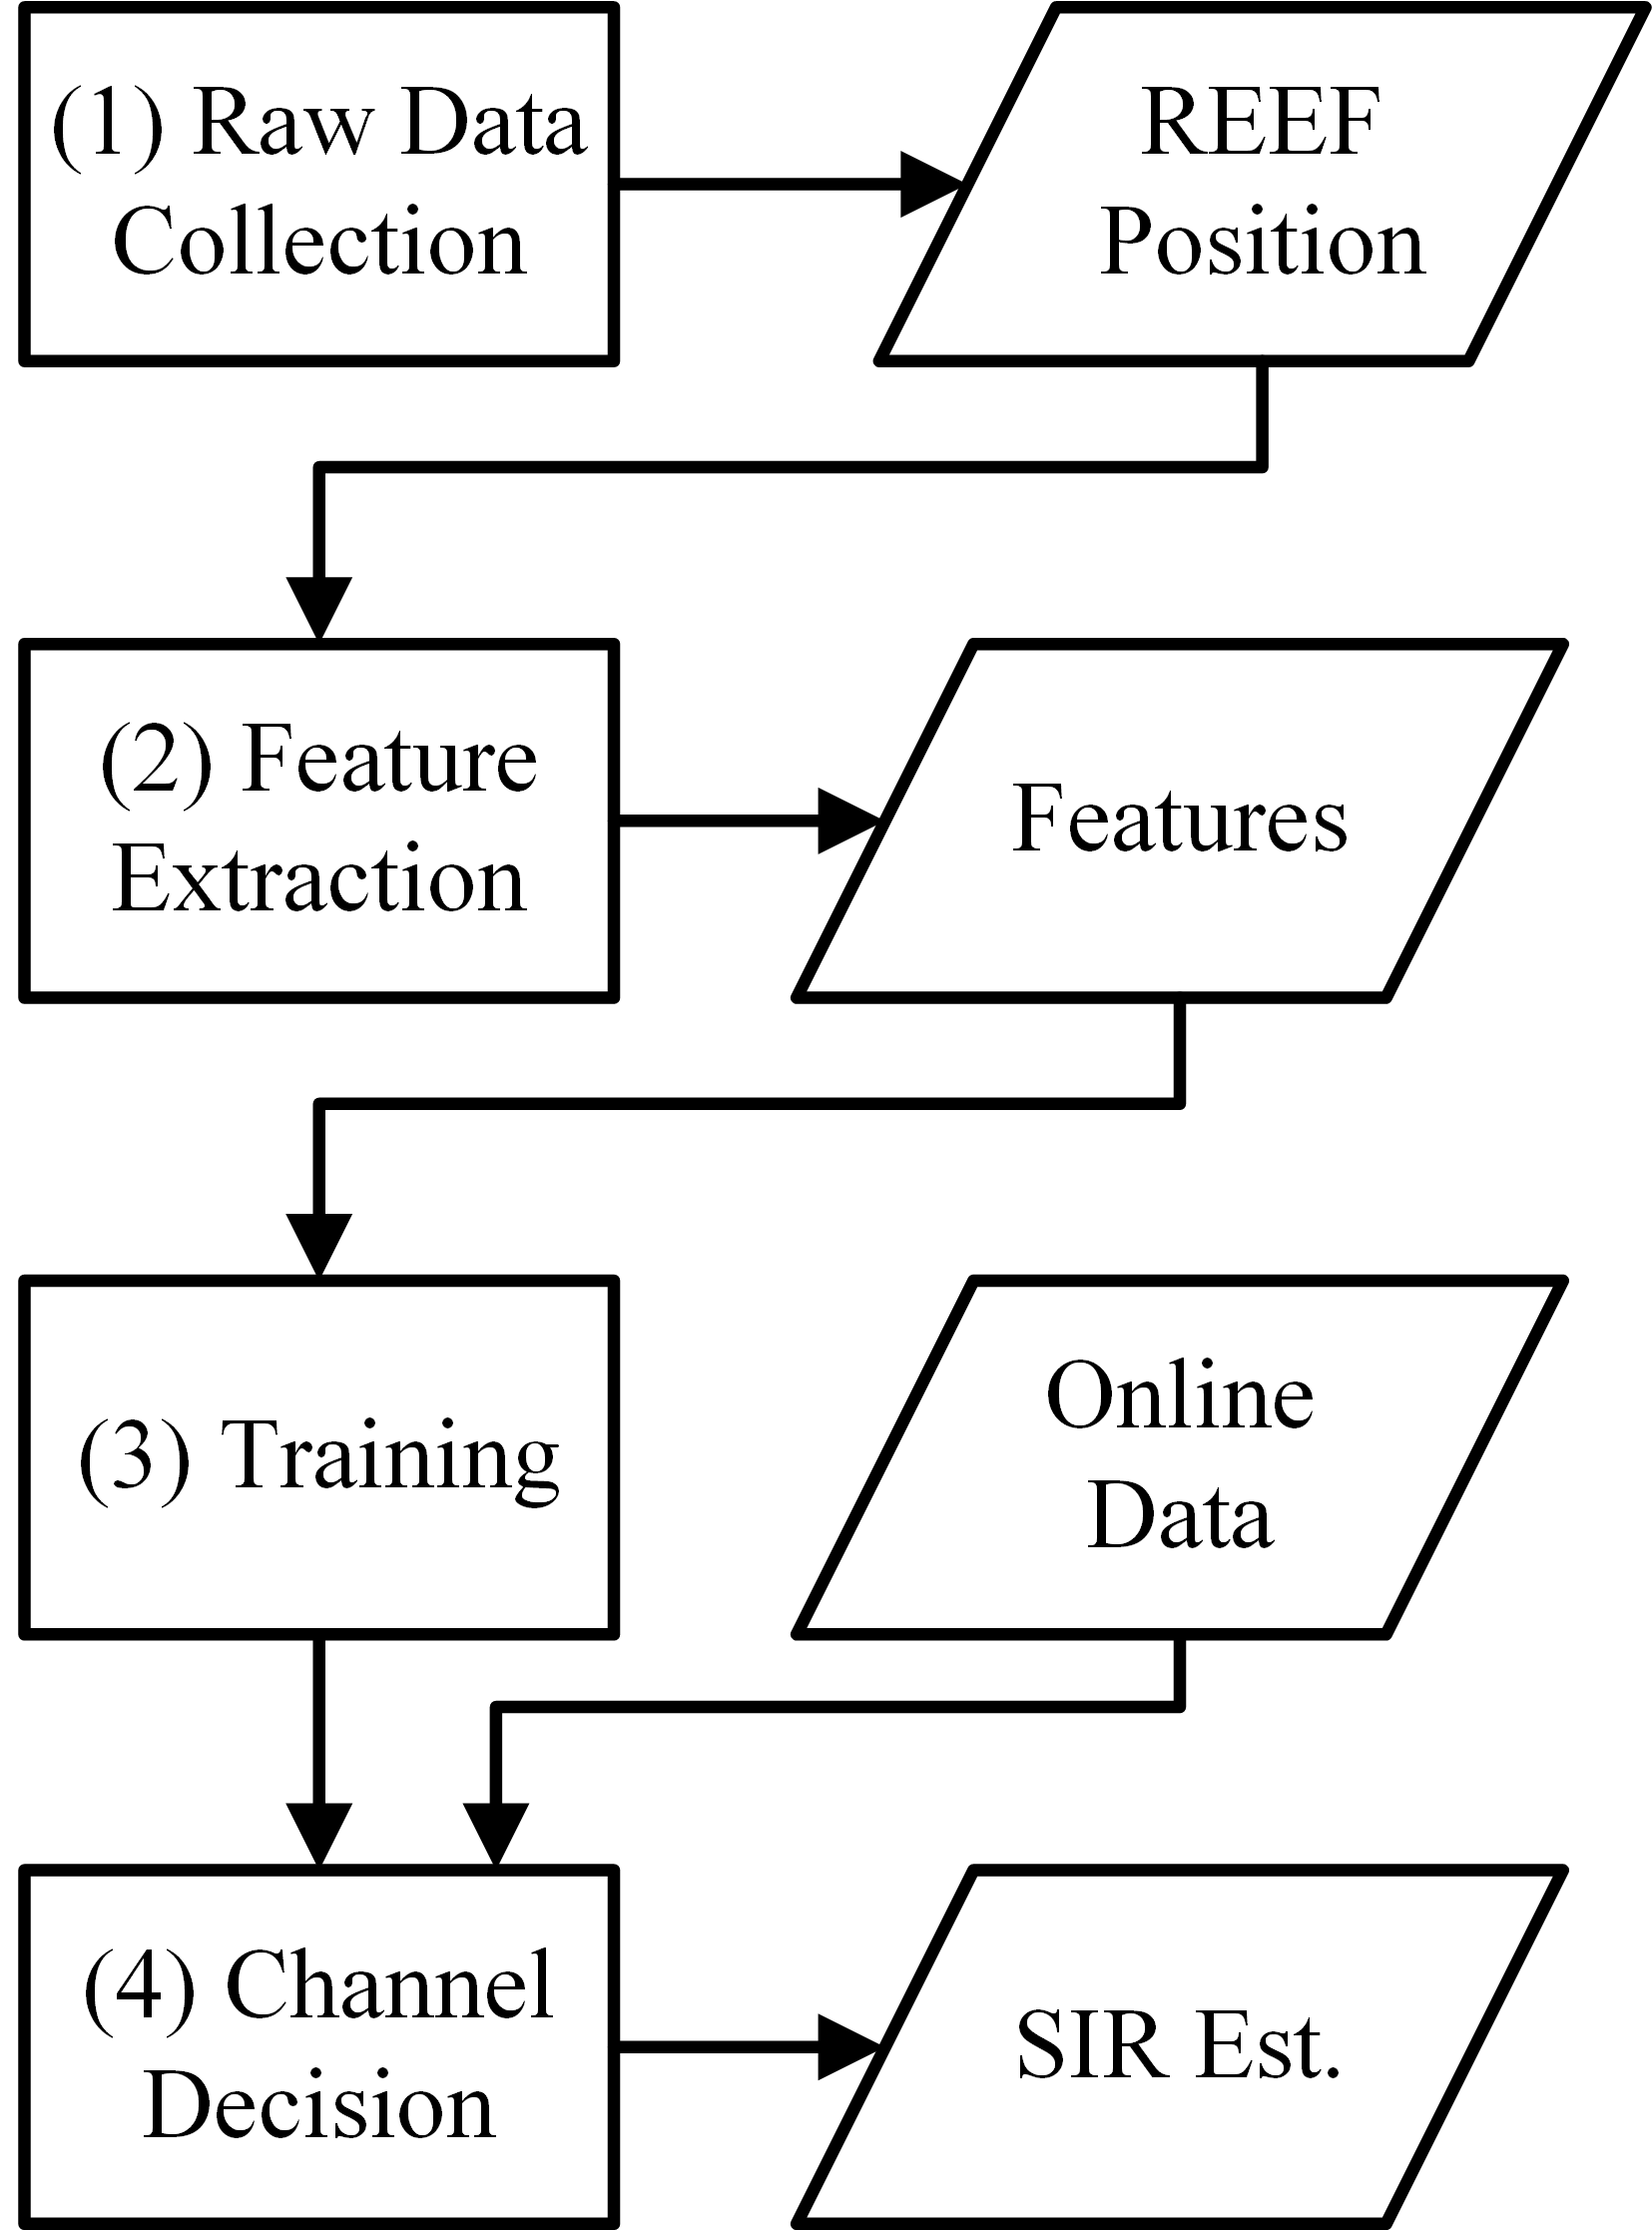
\includegraphics[width=0.65\columnwidth]{diagrams/DataFlow-verticle}
%	    \caption{Data analytics includes raw data capture from a vision system, feature extraction, training, and  operation.}
%	    \label{ftml-conf:fig:dataflow}
%	\end{figure}

The data analysis process for the experiment
%was conducted according to the diagram in Fig.~\ref{ftml-conf:fig:dataflow} and 
is divided into four parts: raw data collection, data cleaning and feature extraction, training, and the operation of the SIR estimation.  The raw data was produced as an output of the \gls{vts} as a time series of z-axis position.  Feature extraction was conducted in MATLAB by following the time series and extracting or calculating features for each iteration.  Once features were extracted, a statistical analysis of the features was conducted to determine the variability of the features as a function of SIR.  Statistical analyses included visual inspection of histograms of each factor and an inspection of the correlation coefficients over the range  of SIRs.  A discussion of the statistical results is provided in~\ref{ftml-conf:sec:results:stats} which demonstrates suitability of the use of position measurements for machine learning. Training of a machine learning algorithm followed. The machine learning algorithm was programmed in Python using the Sci-kit Learn software library.

\subsection{Feature Extraction}\label{ftml-conf:sec:data:feats}

%\begin{figure}[tbp]
% \centering
%	\subfloat[sample time series of probe position\label{ftml-conf:fig:timeseries-zplot}]{%
%		\includegraphics[width=0.8\columnwidth]{plots/timeseries-zplot}}
%	\hfill
%	\subfloat[feature extraction model\label{ftml-conf:fig:timeseriesfeatures}]{%
%		\includegraphics[width=0.9\columnwidth]{diagrams/timeseries.png}}
%	\caption{A time-series sample~\subref{ftml-conf:fig:timeseries-zplot} of a single iteration of the measured z-axis probe position and~\subref{ftml-conf:fig:timeseriesfeatures} the corresponding model for feature extraction.}
%	\label{ftml-conf:fig:timeseries-and-model}      
%\end{figure}	

\begin{figure}[!ht]
	
	\centering
	
	\begin{subfigure}{.95\textwidth}
		\centering
		% include first image
		\includegraphics[]{./chapter-ftml/plots/timeseries-zplot}  
		\caption{sample time series of probe position in mm}
		\label{ftml-conf:fig:timeseries-zplot}
	\end{subfigure}
	
	\begin{subfigure}{.95\textwidth}
		\centering
		% include second image
		\includegraphics[]{./chapter-ftml/diagrams/timeseries.png}  
		\caption{feature extraction model}
		\label{ftml-conf:fig:timeseriesfeatures}
	\end{subfigure}
	
	\caption{A time-series sample~\protect\subref{ftml-conf:fig:timeseries-zplot} of a single iteration of the measured z-axis probe position and~\protect\subref{ftml-conf:fig:timeseriesfeatures} the corresponding model for feature extraction.}
	\label{ftml-conf:fig:timeseries-and-model}
	
\end{figure}

Feature extraction begins with a time series of position of the probe through successive iterations of the plunger applying force to the spring and then returning to its home position.  A sample time series of the z-axis position of the probe is as shown in~Fig.~\ref{ftml-conf:fig:timeseries-zplot}.  Rather than using the time series directly, a more convenient and practical solution is to extract features that represent aspects that may be useful for analysis and machine learning algorithms.  This reduces the number of learning dimensions and usually improves computation efficiency.  The selected features are illustrated in~Fig.~\ref{ftml-conf:fig:timeseriesfeatures}.   Shown in the model, the probe begins at its home position, \textbf{a}.  It will not begin its downward motion until it receives sufficient \gls{fts} readings.  Marker \textbf{b} indicates the beginning of the probes descent.  Marker \textbf{c} represents that point in which the probe descends below a predetermined threshold, and marker \textbf{d} represents the position in which the probe begins its return ascent to the home position.  Finally the probe returns to the home position as indicated by marker \textbf{e}.  Therefore, the extracted features of each successive iteration is defined as follows:

\begin{description}
    \item[Feature $Z_d$] The length of the probe's descent measured in millimeters,
    \item[Feature $\Delta{t}_{ab}$] The duration in seconds the the robot waits before moving the probe along its descent,
    \item[Feature $\Delta{t}_{bc}$] The duration in seconds of the time that the robot takes to move the probe beyond the threshold, $Z_{th}$, of -77 mm,
    \item[Feature $\Delta{t}_{cd}$] The duration in which the probe dwells below $Z_{th}$ and the speed of the probe remains under 0.15 mm/sec,
    \item[Feature $\Delta{t}_{ae}$] The duration of the full iteration as measured from the home position, \textbf{a}, to the next home position, \textbf{e}.
\end{description}


\subsubsection{Statistical Analysis}\label{ftml-conf:sec:data:stats}
Each factor was visually examined to assess its variability as a function of the SIR.  In order to predict the SIR given a set of measurements of the dynamics of the physical system, sufficient variability is needed.  This assessment was performed visually using histograms as a basis for comparison.  The factors $Z_{d}$ and $\Delta{t}_{bc}$ were used for examination of the data using histograms.  

In addition, it would be helpful to show that the factors are uncorrelated as a function of SIR demonstrating a further level of confidence that each factor will be useful to a machine learning algorithm.  This assessment was accomplished by computing the correlation coefficient matrix of the extracted factors as defined by the Pearson product-moment method~\cite{Yeager}.  The correlation coefficient matrix is a covariance matrix that is normalized by the product of the standard deviations of two factors being compared according to $\rho_{X,Y} = cov(X,Y)/(\sigma_{X}\sigma_{Y})$.	Since each factor correlates exactly with itself, a correlation matrix should have values of 1 along the diagonal.  Other elements of the matrix will take on values between -1 and 1.  A visual inspection of the coefficient matrices will show how strongly selected factors vary together.  Correlation can be viewed as a function of SIR to verify that factors are independently applicable to a learning algorithm.  The objective of factor selection is, therefore, to choose factors that are highly uncorrelated and yet still vary appreciably\cite{LeeRodgers1988}.

\subsubsection{Machine Learning}\label{ftml-conf:sec:data:ML}
In order to learn the SIR level from observing the various features, the random forest model is leveraged~\cite{Breiman2001}. Random forest is an ensemble of decision trees with random feature selection which can be used for classification or regression based on the predicted output space. Deploying random forest in machine learning has been successful in various applications such as described in \cite{Zhen2015},~\cite{Shotton2011}, and~\cite{Zhen2014}. Its main advantages are that it is stable, fast to compute, and insusceptible to over-fitting.

In this work, the random forest model is deployed for SIR regression using the five features defined in \ref{ftml-conf:sec:data:feats}. These features are evaluated for each iteration of the probe movement. A data segment is defined which is composed of a number of successive iterations.  The segment size is denoted by $M$. As a result, the random forest regression model is used to get an input vector of size $5M$ and regression output of the corresponding SIR value. The random forest is selected because it is computationally efficient with high-dimensional data and it is robust for outliers and data non-linearity. 

The random forest regression model is first trained by taking a fixed number of segments for each SIR labelled data. The size of the training set for each SIR level is denoted by $T$. The rest of the measurements are used for testing. In general, the proposed machine learning approach will deploy a sliding window approach of size $M$ to collect the features of the force-seeking use case to estimate the current level of SIR at various nodes of the wireless network. 

\subsection{Results} \label{ftml-conf:sec:results}  

The results in this section are  presented from an experimental run in which the jammer \textbf{J} interferes with the router, \textbf{R}, while communication is conducted using a mixed mode of \gls{ieee} 802.11 b and g~\cite{IEEE802.11ac}.  Analyses using histograms and covariance are presented in Section~\ref{ftml-conf:sec:results:stats} followed by results of the machine learning application in Section~\ref{ftml-conf:sec:results-ML}.

\subsubsection{Statistical Analysis}\label{ftml-conf:sec:results:stats}
\paragraph{Analysis of Factors Using Histograms}

%\begin{figure}[tbp]
% \centering
%	\subfloat[z-axis position\label{ftml-conf:fig:results-zpos-hist}]{%
%		\includegraphics[width=0.8\columnwidth]{plots/ZPosHists}}
%	\hfill
%	\subfloat[Plunge delay $\Delta{t}_{bc}$\label{ftml-conf:fig:results-dtbc-hist}]{%
%		\includegraphics[width=0.8\columnwidth]{plots/DeltaTbc.png}}
%	\caption{Variations in probability distributions of the z-axis position \subref{ftml-conf:fig:results-zpos-hist} and the plunge delay \subref{ftml-conf:fig:results-dtbc-hist} indicate that machine learning may be effective in inferring information about the underlying communication channel. In the figure, the baseline case of infinite SIR is depicted as a histogram with white bars, and the experimental case is depicted as a histogram with red bars.}
%	\label{ftml-conf:fig:results-hists}      
%\end{figure}

\begin{figure}[!ht]
	\centering
	\begin{subfigure}{.75\textwidth}
		\centering
		% include first image
		\includegraphics[width=.8\linewidth]{./chapter-ftml/plots/ZPosHists}  
		\caption{z-axis positione}
		\label{ftml-conf:fig:results-zpos-hist}
	\end{subfigure}
	\begin{subfigure}{.75\textwidth}
		\centering
		% include second image
		\includegraphics[width=.8\linewidth]{./chapter-ftml/plots/DeltaTbc.png}  
		\caption{Plunge delay}
		\label{ftml-conf:fig:results-dtbc-hist}
	\end{subfigure}
	\caption{Variations in probability distributions of the z-axis position~\protect\subref{ftml-conf:fig:results-zpos-hist} and the plunge delay~\protect\subref{ftml-conf:fig:results-dtbc-hist} indicate that machine learning may be effective in inferring information about the underlying communication channel. In the figure, the baseline case of infinite SIR is depicted as a histogram with white bars, and the experimental case is depicted as a histogram with red bars.}
	\label{ftml-conf:fig:results-hists}
\end{figure}



The results of the histogram analyses for the z-axis position of the probe and the probe descent delay are shown in Fig.~\ref{ftml-conf:fig:results-zpos-hist} and Fig.~\ref{ftml-conf:fig:results-dtbc-hist}, respectively.  The expectation of the histogram analysis was that $Z_d$ and the $\Delta{T}_{bc}$ would exhibit appreciable variation that may be observed through a visual inspection.  This was indeed the case.  Referring to Fig.~\ref{ftml-conf:fig:results-zpos-hist}, a visual inspection reveals that the minimum z-axis position for each iteration skews to lower positions for lower SIR values and higher positions for higher SIR values.  This implies that the controller algorithm responds faster to force sensor readings at higher SIR values than lower values.  Similarly, by observing the plunge delay, $\Delta{t}_{bc}$, the controller takes more time to respond at lower SIR values than at higher values.  This behavior is exemplified by the probability skew shown in the histograms. 

\paragraph{Factor Correlation Coefficient Analysis}

\begin{table}[!ht]

   	\centering
   	\caption{Correlation Coefficients for $-9\ dB$ SIR}
   	\label{ftml-conf:tab:m9corrcoeff}
   	\begin{tabular}{|l|c|c|c|c|c|}
\hline
&\textbf{$\Delta{t}_{ab}$}&\textbf{$\Delta{t}_{bc}$}&\textbf{$Z_d$}&\textbf{$\Delta{t}_{cd}$}&\textbf{$\Delta{t}_{ae}$}\\\hline
\textbf{$\Delta{t}_{ab}$}&1&0.04&0.04&0&0.56\\\hline
\textbf{$\Delta{t}_{bc}$}&0.04&1&-0.96&-0.08&0.18\\\hline
\textbf{$Z_d$}&0.04&-0.96&1&0.03&-0.01\\\hline
\textbf{$\Delta{t}_{cd}$}&0&-0.08&0.03&1&0\\\hline
\textbf{$\Delta{t}_{ae}$}&0.56&0.18&-0.01&0&1\\\hline
\end{tabular}

   	\vspace{5mm}

   	\centering
   	\caption{Correlation Coefficients for $-8\ dB$ SIR}
   	\label{ftml-conf:tab:m8corrcoeff}
   	\begin{tabular}{|l|c|c|c|c|c|}
\hline
&\textbf{$\Delta{t}_{ab}$}&\textbf{$\Delta{t}_{bc}$}&\textbf{$Z_d$}&\textbf{$\Delta{t}_{cd}$}&\textbf{$\Delta{t}_{ae}$}\\\hline
\textbf{$\Delta{t}_{ab}$}&1&0.01&-0.05&-0.06&0.58\\\hline
\textbf{$\Delta{t}_{bc}$}&0.01&1&-0.99&-0.13&0.1\\\hline
\textbf{$Z_d$}&-0.05&-0.99&1&0.07&-0.1\\\hline
\textbf{$\Delta{t}_{cd}$}&-0.06&-0.13&0.07&1&-0.03\\\hline
\textbf{$\Delta{t}_{ae}$}&0.58&0.1&-0.1&-0.03&1\\\hline
\end{tabular}

   	\vspace{5mm}

   	\centering
   	\caption{Correlation Coefficients for $-7\ dB$ SIR}
   	\label{ftml-conf:tab:m7corrcoeff}
   	\begin{tabular}{|l|c|c|c|c|c|}
\hline
&\textbf{$\Delta{t}_{ab}$}&\textbf{$\Delta{t}_{bc}$}&\textbf{$Z_d$}&\textbf{$\Delta{t}_{cd}$}&\textbf{$\Delta{t}_{ae}$}\\\hline
\textbf{$\Delta{t}_{ab}$}&1&-0.05&-0.04&0.09&0.01\\\hline
\textbf{$\Delta{t}_{bc}$}&-0.05&1&-0.93&-0.17&0.05\\\hline
\textbf{$Z_d$}&-0.04&-0.93&1&0.08&-0.05\\\hline
\textbf{$\Delta{t}_{cd}$}&0.09&-0.17&0.08&1&-0.02\\\hline
\textbf{$\Delta{t}_{ae}$}&0.01&0.05&-0.05&-0.02&1\\\hline
\end{tabular}


\end{table}

Correlation coefficients were calculated for each of the five factors defined in Section~\ref{ftml-conf:sec:data:feats} and correlation coefficients matrices were produced for each of the SIR values used.  The correlation coefficient matrices for SIR values of -9, -8, and -7 are shown in Tables~\ref{ftml-conf:tab:m9corrcoeff}-\ref{ftml-conf:tab:m7corrcoeff}, respectively. Inspection of the correlation coefficient tables indicate that the factors are mostly uncorrelated across SIR values except for the clear correlation between plunge delay and plunge depth. Low correlation values demonstrate a necessary but not sufficient condition for the independent applicability factors to machine learning.  If desired, either $\Delta{t}_{bc}$ or $Z_d$ could be omitted as they are strongly correlated and therefore provide redundant information.

\subsubsection{Machine Learning Results}\label{ftml-conf:sec:results-ML}
The proposed machine learning approach is deployed for three values of the SIR, -9, -8, and -7 dB. First the output of the random forest regression model for two values of the segment size $M$ is shown. The training set size $T=200$ is set for each SIR value. The random forest model is used with a number of estimators of 500 and a tree depth of 5. In Fig.~\ref{ftml-conf:fig:results-BP}, the box plots of the predicted SIRs are presented against the correct value of the corresponding SIR for $M=100$ and $M=1$.  Generally, increasing the value of $M$ increases the acquisition time for the input data for the random forest model while enhancing the performance of the algorithm. By setting $M=1$, it is evident the predicted values of SIR are widely spread around the median and a large number of outliers exists. However, increasing $M$ reduces variations in the predicted SIRs and a smaller number of outliers.


%\begin{figure}[tbp]
%	\subfloat[$M=100$\label{ftml-conf:fig:results-BP-1}]{%
%		\includegraphics[width=\columnwidth]{plots/BP_1}}
%	\hfill
%	\subfloat[$M=1$\label{ftml-conf:fig:results-BP-2}]{%
%		\includegraphics[width=\columnwidth]{plots/BP_2}}
%	\caption{Predicted SIR versus actual SIR for the cases of~\subref{ftml-conf:fig:results-BP-1} $M=100$ and~\subref{ftml-conf:fig:results-BP-2} $M=1$. The box plots show the median value while the bottom and top edges of the box indicate the 25th and 75th percentiles.  Statistical outliers are shown as red $+$ signs.}
%	\label{ftml-conf:fig:results-BP}      
%\end{figure}

\begin{figure}[!ht]
	\begin{subfigure}{.5\textwidth}
		\centering
		% include first image
		\includegraphics[width=.8\linewidth]{./chapter-ftml/plots/BP_1}  
		\caption{[$M=100$}
		\label{ftml-conf:fig:results-BP-1}
	\end{subfigure}
	\begin{subfigure}{.5\textwidth}
		\centering
		% include second image
		\includegraphics[width=.8\linewidth]{./chapter-ftml/plots/BP_2}  
		\caption{[$M=1$}
		\label{ftml-conf:fig:results-BP-2}
	\end{subfigure}
	\caption{Predicted SIR versus actual SIR for the cases of~\protect\subref{ftml-conf:fig:results-BP-1} $M=100$ and~\protect\subref{ftml-conf:fig:results-BP-2} $M=1$. The box plots show the median value while the bottom and top edges of the box indicate the 25th and 75th percentiles.  Statistical outliers are shown as red $+$ signs.}
	\label{ftml-conf:fig:results-BP}
\end{figure}

In Fig.~\ref{ftml-conf:fig:prediction-error}, the two criteria for measuring the performance of the proposed SIR estimation algorithm is presented. The performance against the segment size $M$ is shown. The first criterion is the mean squared error where the mean of the squared error between the estimated \gls{sir} and the actual \gls{sir} values is calculated. The second criterion is the variance score which is a statistical measure of how close the data are to the fitted regression line. The r-squared variance score is used which is defined as the ratio between the total variance explained by model and total variance of the data \cite{r-squared}. In this figure the improvement in the performance against the segment size is demonstrated. 

\begin{figure}[tbp]
 \centering
 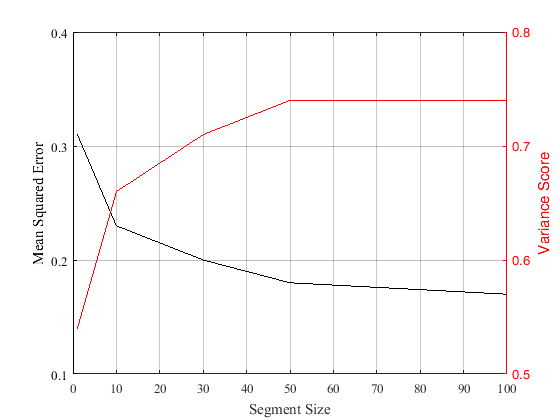
\includegraphics[width=0.75\columnwidth]{./chapter-ftml/plots/prediction-error}
 \caption{The performance of the random forest regression model against $M$.}
 \label{ftml-conf:fig:prediction-error}
\end{figure}

\subsection{Conclusion}\label{ftml-conf:sec:conclusion}

This investigation presented a practical use case of a wireless force-torque feedback control system that could be deployed in a manufacturing assembly system such as a pick-and-place or assembly operation.  A 6-\gls{dof} force sensor was connected to a robot controller tasked with moving a probe along a linear path until an opposing force exceeding 5 N was detected.  It is demonstrated that the reliability of the wireless communication system directly impacts the repeatability performance of the physical system. It is also demonstrated that the quality of the underlying wireless channel may be inferred by observing the position of the probe along a single spatial dimension and applying machine learning to predict the \gls{sir}. The findings provide motivation for applying machine learning to larger more complex systems with high degrees of freedom. Future work will extend to the inclusion of more descriptive factors, the addition of network information such as the wireless protocol mode, and the addition of a larger number of variables tracked by many remote observers. Experimentation with neural networks and deep learning to improve prediction accuracy and better generalization will be of great values to wireless operations in factories.  Finally, the applications of online machine learning techniques to this and other use cases could provide significant benefits to the manufacturing community.




	\section{Subsequent Investigations}

The contents of this section explain the subsequent analysis explanding on the approach, methodology, and results of the initial investigations using machine learning to infer the signal-to-interference of a single radio link using situational awareness information from a camera system as published in~\cite{CandellISIE2019.Conf}.  In this further investigation, the performance of the machine learning algorithms themselves were investigated to determine optimal selection given the particular use case. Publication is forthcoming~\cite{Candell2020.Jrnl.Access}.


\subsection{Data Analysis}\label{ftml-jrnl:sec:dataanalysis}

%	\begin{figure}[tbp]
%	    \centering
%	    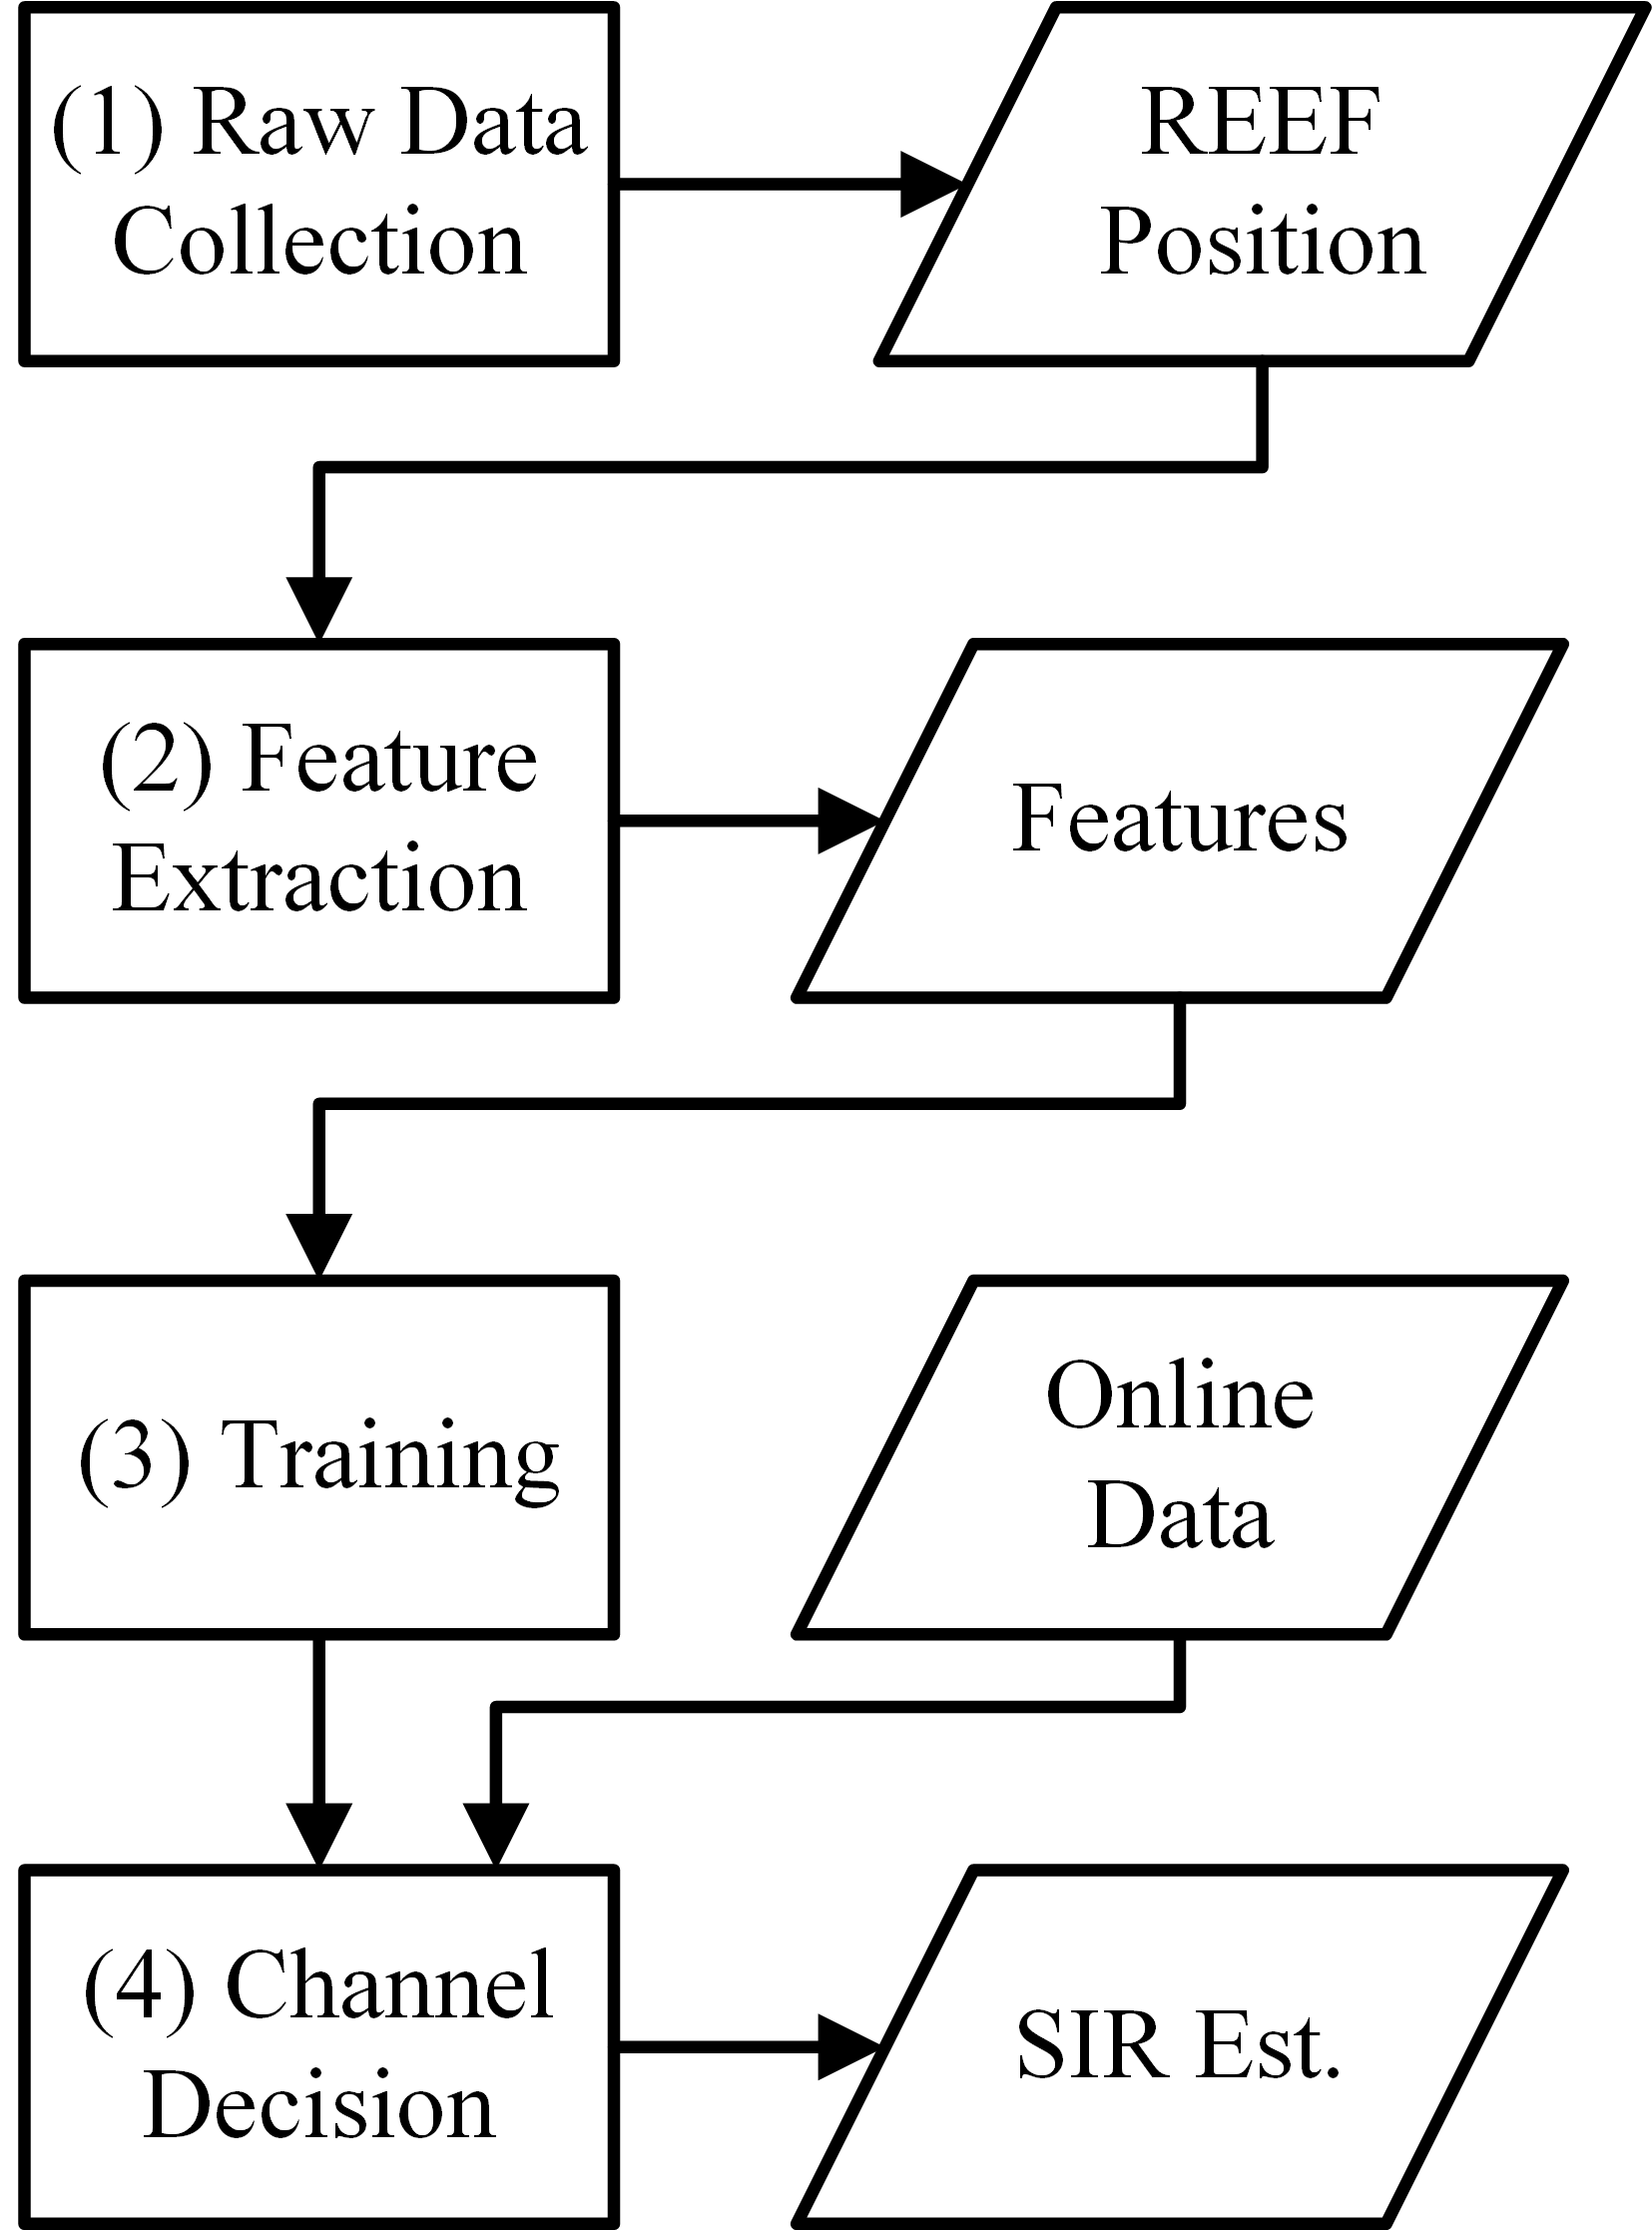
\includegraphics[width=0.65\columnwidth]{diagrams/DataFlow-verticle}
%	    \caption{Data analytics includes raw data capture from a vision system, feature extraction, training, and  operation.}
%	    \label{ftml-jrnl:fig:dataflow}
%	\end{figure}

The data analysis process for the experiment
%was conducted according to the diagram in Fig.~\ref{ftml-jrnl:fig:dataflow} and 
is divided into four parts: raw data collection, data cleaning and feature extraction, training, and the operation of the SIR estimation. The raw data was produced as an output of the VTS as a time series of z-axis position. Feature extraction was conducted in MATLAB by following the time series and extracting or calculating features for each iteration.  Once features were extracted, a statistical analysis of the features was conducted to determine the variability of the features as a function of SIR \cite{Candell_ISIT_2019}. Training of a machine learning algorithm followed. The machine learning algorithm was programmed in Python using the Sci-kit Learn library~\cite{SCIKITLEARN}.

\subsubsection{Feature Extraction}\label{ftml-jrnl:sec:data:feats}

Refer to Section~\ref{ftml-conf:sec:data:feats} for a discussion on how features used for training were extracted.  As stated in the previous discussion, rather than using the entire time series directly, a more convenient and practical solution is to extract features that represent aspects that may be useful for analysis and machine learning algorithms.  By using features rather than the time series, we reduce the number of learning dimensions and usually improve computation efficiency.  The selected features are illustrated in Fig.~\ref{ftml-conf:fig:timeseriesfeatures}.

%\begin{figure}[tbp]
%	\centering
%	\subfloat[sample time series of probe position in mm\label{ftml-jrnl:fig:timeseries-zplot}]{%
%		\includegraphics[width=0.75\columnwidth]{plots/timeseries-zplot}}
%	\hfill
%	\subfloat[feature extraction model\label{ftml-jrnl:fig:timeseriesfeatures}]{%
%		\includegraphics[width=0.8\columnwidth]{diagrams/timeseries.png}}
%	\caption{A time-series sample~\subref{ftml-jrnl:fig:timeseries-zplot} of a single iteration of the measured z-axis probe position and~\subref{ftml-jrnl:fig:timeseriesfeatures} the corresponding model for feature extraction.}
%	\label{ftml-jrnl:fig:timeseries-and-model}      
%\end{figure}

%\begin{figure}[!ht]
%	\centering
%	
%	\begin{subfigure}{.65\textwidth}
%		\centering
%		% include first image
%		\includegraphics[width=.8\linewidth]{./chapter-ftml/plots/timeseries-zplot}  
%		\caption{sample time series of probe position in mm}
%		\label{ftml-jrnl:fig:timeseries-zplot}
%	\end{subfigure}
%
%	\begin{subfigure}{.75\textwidth}
%		\centering
%		% include second image
%		\includegraphics[width=.8\linewidth]{./chapter-ftml/diagrams/timeseries.png}  
%		\caption{feature extraction model}
%		\label{ftml-jrnl:fig:timeseriesfeatures}
%	\end{subfigure}
%
%	\caption{A time-series sample~\protect\subref{ftml-jrnl:fig:timeseries-zplot} of a single iteration of the measured z-axis probe position and~\protect\subref{ftml-jrnl:fig:timeseriesfeatures} the corresponding model for feature extraction.}
%	\label{ftml-jrnl:fig:timeseries-and-model}
%	
%\end{figure}	

%A sample time series of the z-axis position of the probe is as shown in~Fig.~\ref{ftml-jrnl:fig:timeseries-zplot}.  Rather than using the time series directly, a more convenient and practical solution is to extract features that represent aspects that may be useful for analysis and machine learning algorithms. The selected features are illustrated in~Fig.~\ref{ftml-jrnl:fig:timeseriesfeatures}. Shown in the model, the probe begins at its home position, \textbf{a}.  It will not begin its downward motion until it receives sufficient FTS readings.  Marker \textbf{b} indicates the beginning of the probes descent.  Marker \textbf{c} represents that point in which the probe descends below a predetermined threshold, and marker \textbf{d} represents the position in which the probe begins its return ascent to the home position.  Finally the probe returns to the home position as indicated by marker \textbf{e}.  Therefore, the extracted features of each successive iteration is defined as follows:
%
%\begin{description}
%	\item[Feature $Z_d$] The length of the probe's descent measured in millimeters,
%	\item[Feature $\Delta{t}_{ab}$] The duration in seconds the the robot waits before moving the probe along its descent,
%	\item[Feature $\Delta{t}_{bc}$] The duration in seconds of the time that the robot takes to move the probe beyond the threshold, $Z_{th}$, of -77 mm,
%	\item[Feature $\Delta{t}_{cd}$] The duration in which the probe dwells below $Z_{th}$ and the speed of the probe remains under 0.15 mm/sec,
%	\item[Feature $\Delta{t}_{ae}$] The duration of the full iteration as measured from the home position, \textbf{a}, to the next home position, \textbf{e}.
%\end{description}

\subsubsection{ML-based SIR Estimation}\label{ftml-jrnl:sec:data:ML}
In order to learn the SIR level from observing the various features, it is possible to leverage supervised machine learning regression schemes. 
%the random forest model \cite{RF}. Random forest is an ensemble of decision trees with random feature selection which can be used for classification or regression based on the predicted output space. Deploying random forest in machine learning has been successful in various applications such as \cite{RF_1,RF_2,RF_3}. Its main advantages are that it is stable, fast to compute, and insusceptible to over-fitting.
This work compares the deployment of various machine learning algorithms for SIR regression using the five features defined in \ref{ftml-jrnl:sec:data:feats}. These features are evaluated for each iteration of the probe movement. A data segment is defined as a number of successive iterations and the segment size is denoted by $M$. As a result, each regression model is used to get an input vector of size $5M$ and the regression output of the corresponding SIR value. 
%The random forest is selected because it is computationally efficient with high-dimensional data and it is robust for outliers and data non-linearity. 

One starts by training each regression model by taking a fixed number of segments for each SIR labeled data. The size of the training set for each SIR level is denoted by $T$. The rest of the measurements are used for testing. In general, the proposed machine learning approach will deploy a sliding window approach of size $M$ to collect the features of the force-seeking use case to estimate the current level of SIR at various nodes of the wireless network. 

\subsection{Results} \label{ftml-jrnl:sec:results}  
In this section, the experimental results for 4 different settings are considered. The four settings are defined as follows: i) setting b/g-Router: the jamming signal impacts the router and IEEE 802.11 b/g is deployed ~\cite{IEEE802.11ac}, ii) setting b/g-Station: the jamming signal impacts the station and IEEE 802.11 b/g is deployed, iii) setting b/g/n-Router: the jamming signal impacts the router and IEEE 802.11 b/g/n is deployed, and iv) setting b/g/n-Station: the jamming signal impacts the station and IEEE 802.11 b/g/n is deployed.  

When the jamming signal has an impact on the router, this work considers 3 values of the SIR which are -9, -8, -7 dB while having 1, 2, 3 dB for the settings in which jamming has an impact on the station. Except otherwise mentioned, $M = 50$ and $T = 200$ are used. 

\subsubsection{Machine Learning Algorithm Comparison}
In this subsection, various regression approaches are compared using two performance criteria, namely, the mean squared error (MSE)\eqref{eq:scikit:MSE} and the R-squared variance score\eqref{eq:scikit:R2variance}~\cite{r-squared}. R-squared variance score indicates the percentage of the variance in the dependent variable that the independent variables explain collectively.  It is equivalent to how R-sqaured is used in financial investments to explain how one security explains the performance of an entire portfolio. The used version of R-squared in the Sci-kit Learn library measures the strength of the relationship between the model used and the dependent variable on a convenient -1 to 1 scale.  The best possible outcome is 1 when predicted values capture the variance of the independent variable. It takes a value of 0 when the predicted value is constant and negative values when the regression model cannot follow the trend of the data. The performance for different values of $M$ is presented. The compared algorithms are the random forest, gradient boosting, extreme gradient boosting (XGBM), decision tree, support vector machine (SVM), k-nearest neighbor, kernel ridge, and linear ridge \cite{SCIKITLEARN,Chen:2016:XST:2939672.2939785}. %xxxx references needed

\begin{equation}
\text{MSLE}(y, \hat{y}) = \frac{1}{n_\text{samples}} \sum_{i=0}^{n_\text{samples} - 1} (\log_e (1 + y_i) - \log_e (1 + \hat{y}_i) )^2.
\label{eq:scikit:MSE}
\end{equation}

\begin{equation}
R^2(y, \hat{y}) = 1 - \frac{\sum_{i=1}^{n} (y_i - \hat{y}_i)^2}{\sum_{i=1}^{n} (y_i - \bar{y})^2}
\label{eq:scikit:R2variance}
\end{equation}

% Table generated by Excel2LaTeX from sheet 'ML_Regression_MSE'
\begin{table}[!ht]
	\centering
	\caption{MSE values of various ML algorithms for jamming setting b/g-Router}
	\begin{tabular}{|p{5.3em}|c|c|c|c|c|}
		\toprule
		& \multicolumn{1}{p{2.4em}|}{M = 1} & \multicolumn{1}{p{2.9em}|}{M = 10} & \multicolumn{1}{p{2.9em}|}{M = 30} & \multicolumn{1}{p{2.9em}|}{M = 50} & \multicolumn{1}{p{3.4em}|}{M = 100} \\
		\midrule
		Random Forest	 & 0.61  & 0.54  & 0.49  & 0.48  & 0.46 \\
		\midrule
		Gradient Boosting  & 0.56  & 0.55  & 0.47  & 0.45  & 0.44 \\
		\midrule
		XGBM  & 0.62  & 0.53  & 0.45  & 0.43  & 0.41 \\
		\midrule
		Decission Tree & 1.07  & 0.99  & 0.87  & 0.91  & 0.97 \\
		\midrule
		SVM   & 0.92  & 0.99  & 0.98  & 0.97  & 0.96 \\
		\midrule
		KNN   & 0.73  & 0.74  & 0.73  & 0.74  & 0.77 \\
		\midrule
		Kernal Ridge & 0.97  & 0.73  & 0.71  & 0.71  & 0.71 \\
		\midrule
		Linear Ridge & 0.7   & 0.7   & 0.7   & 0.71  & 0.71 \\
		\bottomrule
	\end{tabular}%
	\label{ftml-jrnl:tab:T1}%
\end{table}%

In Table~\ref{ftml-jrnl:tab:T1}, the MSE performance of various algorithms are presented for setting a 802.11 b/g mode setting at the router. The ensemble-based algorithms, which are the random forest, gradient boosting, and XGBM, perform better than non-ensemble algorithms. This happens because the ensemble-based algorithms learn from the training data without having an initial model to fit thus allowing for capturing the randomness impacts on the collected data. Moreover, the XGBM gives slightly better performance than the random forest and gradient boosting algorithms except at $M=1$. The XGBM performs gradient boosting over random set of trees and hence the superior performance. It also has superior variance score as well in Table~\ref{ftml-jrnl:tab:T2}. Generally, in Table~\ref{ftml-jrnl:tab:T2}, similar trends as Table~\ref{ftml-jrnl:tab:T1} can be found for various machine learning algorithms where ensemble-based algorithms have the best performance among others and their performance is enhanced by increasing the segment size $M$ of the measured data.

% Table generated by Excel2LaTeX from sheet 'ML_Regression_R2'
\begin{table}[!ht]
	\centering
	\caption{Variance score values of various ML algorithms for jamming setting b/g-Router}
	\begin{tabular}{|p{5.3em}|c|c|c|c|c|}
		\toprule
		& \multicolumn{1}{p{2.4em}|}{M = 1} & \multicolumn{1}{p{2.9em}|}{M = 10} & \multicolumn{1}{p{2.9em}|}{M = 30} & \multicolumn{1}{p{2.9em}|}{M = 50} & \multicolumn{1}{p{3.4em}|}{M = 100} \\
		\midrule
		Random Forest	 & 0.15  & 0.2   & 0.3   & 0.35  & 0.35 \\
		\midrule
		Gradient Boosting  & 0.02  & 0.2   & 0.34  & 0.37  & 0.42 \\
		\midrule
		XGBM  & 0.12  & 0.25  & 0.36  & 0.4   & 0.43 \\
		\midrule
		Decission Tree & -0.57 & -0.44 & -0.36 & -0.3  & -0.22 \\
		\midrule
		SVM   & -0.34 & -0.38 & -0.37 & -0.37 & -0.32 \\
		\midrule
		KNN   & -0.05 & -0.02 & -0.02 & -0.08 & -0.04 \\
		\midrule
		Kernal Ridge & -0.48 & -0.05 & 0     & 0     & 0 \\
		\midrule
		Linear Ridge & 0.01  & 0.01  & 0     & -0.01 & 0 \\
		\bottomrule
	\end{tabular}%
	\label{ftml-jrnl:tab:T2}%
\end{table}%


% Table generated by Excel2LaTeX from sheet 'ML_Regression_MSE'
% \begin{table}[htbp]
%   \centering
%   \caption{MSE Values of various ML algorithms for setting 2}
%     \begin{tabular}{|p{6.7em}|c|c|c|c|c|}
%     \toprule
%           & \multicolumn{1}{p{3em}|}{M = 1} & \multicolumn{1}{p{3em}|}{M = 10} & \multicolumn{1}{p{3em}|}{M = 30} & \multicolumn{1}{p{3em}|}{M = 50} & \multicolumn{1}{p{3.5em}|}{M = 100} \\
%     \midrule
%     Random Forest	 & 0.31  & 0.23  & 0.2   & 0.18  & 0.17 \\
%     \midrule
%     Gradient Boosting  & 0.32  & 0.16  & 0.14  & 0.14  & 0.14 \\
%     \midrule
%     XGBM  & 0.3   & 0.17  & 0.12  & 0.1   & 0.1 \\
%     \midrule
%     Decission Tree & 0.6   & 0.48  & 0.46  & 0.44  & 0.39 \\
%     \midrule
%     SVM   & 0.96  & 0.96  & 0.94  & 0.95  & 0.88 \\
%     \midrule
%     KNN   & 0.76  & 0.73  & 0.7   & 0.71  & 0.73 \\
%     \midrule
%     Kernal Ridge & 4.9   & 1.08  & 0.69  & 0.44  & 0.39 \\
%     \midrule
%     Linear Ridge & 0.67  & 0.67  & 0.67  & 0.67  & 0.66 \\
%     \bottomrule
%     \end{tabular}%
%   \label{ftml-jrnl:tab:addlabel}%
% \end{table}%

% % Table generated by Excel2LaTeX from sheet 'ML_Regression_R2'
% \begin{table}[htbp]
%   \centering
%   \caption{variance Score Values of various ML algorithms for setting 2}
%     \begin{tabular}{|p{6.7em}|c|c|c|c|c|}
%     \toprule
%           & \multicolumn{1}{p{3em}|}{M = 1} & \multicolumn{1}{p{3em}|}{M = 10} & \multicolumn{1}{p{3em}|}{M = 30} & \multicolumn{1}{p{3em}|}{M = 50} & \multicolumn{1}{p{3.5em}|}{M = 100} \\
%     \midrule
%     Random Forest	 & 0.54  & 0.69  & 0.74  & 0.74  & 0.76 \\
%     \midrule
%     Gradient Boosting  & 0.49  & 0.71  & 0.8   & 0.79  & 0.81 \\
%     \midrule
%     XGBM  & 0.56  & 0.77  & 0.83  & 0.85  & 0.85 \\
%     \midrule
%     Decission Tree & 0.14  & 0.31  & 0.34  & 0.36  & 0.35 \\
%     \midrule
%     SVM   & -0.45 & -0.39 & -0.46 & -0.43 & -0.36 \\
%     \midrule
%     KNN   & -0.08 & -0.06 & -0.07 & -0.11 & -0.09 \\
%     \midrule
%     Kernal Ridge & -5.98 & -0.62 & -0.07 & -0.04 & 0.02 \\
%     \midrule
%     Linear Ridge & 0     & 0     & 0     & 0     & -0.01 \\
%     \bottomrule
%     \end{tabular}%
%   \label{ftml-jrnl:tab:addlabel}%
% \end{table}%

% 	% Table generated by Excel2LaTeX from sheet 'ML_Regression_MSE'
% \begin{table}[htbp]
%   \centering
%   \caption{MSE Values of various ML algorithms for setting 3}
%     \begin{tabular}{|p{6.7em}|c|c|c|c|c|}
%     \toprule
%           & \multicolumn{1}{p{3em}|}{M = 1} & \multicolumn{1}{p{3em}|}{M = 10} & \multicolumn{1}{p{3em}|}{M = 30} & \multicolumn{1}{p{3em}|}{M = 50} & \multicolumn{1}{p{3.5em}|}{M = 100} \\
%     \midrule
%     Random Forest	 & 0.49  & 0.37  & 0.31  & 0.29  & 0.27 \\
%     \midrule
%     Gradient Boosting  & 0.58  & 0.36  & 0.25  & 0.24  & 0.18 \\
%     \midrule
%     XGBM  & 0.53  & 0.35  & 0.25  & 0.2   & 0.15 \\
%     \midrule
%     Decission Tree & 1.03  & 0.84  & 0.82  & 0.69  & 0.73 \\
%     \midrule
%     SVM   & 0.94  & 0.95  & 0.86  & 0.89  & 0.83 \\
%     \midrule
%     KNN   & 0.67  & 0.67  & 0.67  & 0.67  & 0.73 \\
%     \midrule
%     Kernal Ridge & 0.62  & 0.63  & 0.6   & 0.6   & 0.61 \\
%     \midrule
%     Linear Ridge & 0.6   & 0.6   & 0.61  & 0.61  & 0.63 \\
%     \bottomrule
%     \end{tabular}%
%   \label{ftml-jrnl:tab:addlabel}%
% \end{table}%

% 	% Table generated by Excel2LaTeX from sheet 'ML_Regression_R2'
% \begin{table}[htbp]
%   \centering
%   \caption{variance Score Values of various ML algorithms for setting 3}
%     \begin{tabular}{|p{6.7em}|c|c|c|c|c|}
%     \toprule
%           & \multicolumn{1}{p{3em}|}{M = 1} & \multicolumn{1}{p{3em}|}{M = 10} & \multicolumn{1}{p{3em}|}{M = 30} & \multicolumn{1}{p{3em}|}{M = 50} & \multicolumn{1}{p{3.5em}|}{M = 100} \\
%     \midrule
%     Random Forest	 & 0.12  & 0.35  & 5     & 0.5   & 0.56 \\
%     \midrule
%     Gradient Boosting  & 0.02  & 0.39  & 0.53  & 0.6   & 0.67 \\
%     \midrule
%     XGBM  & 0.16  & 0.45  & 0.6   & 0.66  & 0.73 \\
%     \midrule
%     Decission Tree & -0.79 & -0.38 & -0.33 & -0.26 & -0.16 \\
%     \midrule
%     SVM   & -0.56 & -0.6  & -0.55 & -0.52 & -0.41 \\
%     \midrule
%     KNN   & -0.15 & -0.13 & -0.14 & -0.1  & -0.24 \\
%     \midrule
%     Kernal Ridge & -0.41 & -0.04 & -0.01 & -0.02 & -0.03 \\
%     \midrule
%     Linear Ridge & 0     & -0.01 & -0.03 & -0.05 & -0.09 \\
%     \bottomrule
%     \end{tabular}%
%   \label{ftml-jrnl:tab:addlabel}%
% \end{table}%

Similarly, in Table~\ref{ftml-jrnl:tab:T3}, the ensemble-based algorithms perform better than other algorithms and the XGBM is the best among them. In this setting b/g/n-Station, the interference impacts the router and hence the MSE values generally higher than the corresponding cases in setting b/g-Router. In this case, the interference has a larger impact and hence larger MSE. That leads to larger distinction between the performance of the machine learning algorithms. 
% Table generated by Excel2LaTeX from sheet 'ML_Regression_MSE'
\begin{table}[!ht]
	\centering
	\caption{MSE values of various ML algorithms for jamming setting b/g-Station}
	\begin{tabular}{|p{5.3em}|c|c|c|c|c|}
		\toprule
		& \multicolumn{1}{p{2.4em}|}{M = 1} & \multicolumn{1}{p{2.9em}|}{M = 10} & \multicolumn{1}{p{2.9em}|}{M = 30} & \multicolumn{1}{p{2.9em}|}{M = 50} & \multicolumn{1}{p{3.4em}|}{M = 100} \\
		\midrule
		Random Forest	 & 0.88  & 0.79  & 0.76  & 0.69  & 0.7 \\
		\midrule
		Gradient Boosting  & 0.95  & 0.71  & 0.61  & 0.56  & 0.56 \\
		\midrule
		XGBM  & 0.85  & 0.73  & 0.59  & 0.52  & 0.48 \\
		\midrule
		Decission Tree & 1.48  & 1.46  & 1.33  & 1.33  & 1.32 \\
		\midrule
		SVM   & 1.34  & 1.36  & 1.36  & 1.39  & 1.49 \\
		\midrule
		KNN   & 1.01  & 1.04  & 1.03  & 1.05  & 1.13 \\
		\midrule
		Kernal Ridge & 4.42  & 1.25  & 0.98  & 0.97  & 0.99 \\
		\midrule
		Linear Ridge & 0.93  & 0.94  & 0.94  & 0.95  & 0.99 \\
		\bottomrule
	\end{tabular}%
	\label{ftml-jrnl:tab:T3}%
\end{table}%

% 	% Table generated by Excel2LaTeX from sheet 'ML_Regression_R2'
% \begin{table}[htbp]
%   \centering
%   \caption{variance Score Values of various ML algorithms for setting 4}
%     \begin{tabular}{|p{6.7em}|c|c|c|c|c|}
%     \toprule
%           & \multicolumn{1}{p{3em}|}{M = 1} & \multicolumn{1}{p{3em}|}{M = 10} & \multicolumn{1}{p{3em}|}{M = 30} & \multicolumn{1}{p{3em}|}{M = 50} & \multicolumn{1}{p{3.5em}|}{M = 100} \\
%     \midrule
%     Random Forest	 & 0.08  & 0.15  & 0.22  & 0.27  & 0.3 \\
%     \midrule
%     Gradient Boosting  & -0.04 & 0.23  & 0.39  & 0.43  & 0.44 \\
%     \midrule 
%     XGBM  & 0.07  & 0.21  & 0.37  & 0.46  & 0.53 \\
%     \midrule
%     Decission Tree & -0.51 & -0.49 & -0.42 & -0.39 & -0.48 \\
%     \midrule
%     SVM   & -0.44 & -0.51 & -0.44 & -0.46 & -0.52 \\
%     \midrule
%     KNN   & -0.12 & -0.13 & -0.1  & -0.09 & -0.12 \\
%     \midrule
%     Kernal Ridge & -3.61 & -0.26 & -0.05 & 0     & 0 \\
%     \midrule
%     Linear Ridge & 0     & -0.01 & 0     & 0     & 0 \\
%     \bottomrule
%     \end{tabular}%
%   \label{ftml-jrnl:tab:addlabel}%
% \end{table}%

\subsubsection{Tuning the Random Forest and Gradient Boosting Regressors}

In this subsection, the impacts of the number of estimators and the depth for gradient boosting and random forest algorithms are studied. The XGBM parameters are optimized automatically when the function is called to be executed. The work shows that the MSE performance results for setting b/g-Router while same trend holds for other system settings as well. 

For random forest algorithm, Table~\ref{ftml-jrnl:tab:T4} shows that the tree depth has more impact on the performance than the number of the estimators (\# est.). However, increasing the depth improves the performance till the value of 5 where increasing the depth cause slight improvements.   
% Table generated by Excel2LaTeX from sheet 'ML_Random_Forest_MSE_Matrix'
\begin{table}[!ht]
	\centering
	\caption{MSE of Random Forrest regression parameters for jamming setting b/g-Router}
	\begin{tabular}{|c|c|c|c|c|c|c|}
		\toprule
		\backslashbox{Depth}{\# est.}
		
		& 100   & 200   & 300   & 400   & 500   & 600 \\
		\midrule
		1     & 0.64  & 0.64  & 0.64  & 0.63  & 0.63  & 0.63 \\
		\midrule
		3     & 0.53  & 0.53  & 0.53  & 0.53  & 0.53  & 0.52 \\
		\midrule
		5     & 0.5   & 0.5   & 0.5   & 0.48  & 0.48  & 0.48 \\
		\midrule
		7     & 0.49  & 0.49  & 0.48  & 0.48  & 0.48  & 0.48 \\
		\midrule
		9     & 0.48  & 0.48  & 0.47  & 0.47  & 0.47  & 0.47 \\
		\bottomrule
	\end{tabular}%
	\label{ftml-jrnl:tab:T4}%
\end{table}%

For gradient boosting, Table~\ref{ftml-jrnl:tab:T5} shows that a similar trend as a random forest exists where depth has a larger impact on the performance. However, increasing the depth more than 7 causes the MSE performance to degrade significantly. 

% Table generated by Excel2LaTeX from sheet 'ML_Gradient_Boosting__MSE_Matri'
\begin{table}[!ht]
	\centering
	\caption{MSE of Gradient Boosting regression parameters for jamming setting b/g-Router}
	\begin{tabular}{|c|c|c|c|c|c|c|}
		\toprule
		\backslashbox{Depth}{\# est.}
		& 100   & 200   & 300   & 400   & 500   & 600 \\
		\midrule
		1     & 0.48  & 0.47  & 0.46  & 0.46  & 0.45  & 0.46 \\
		\midrule
		3     & 0.47  & 0.47  & 0.47  & 0.47  & 0.46  & 0.47 \\
		\midrule
		5     & 0.48  & 0.47  & 0.47  & 0.47  & 0.47  & 0.47 \\
		\midrule
		7     & 0.48  & 0.48  & 0.48  & 0.48  & 0.46  & 0.49 \\
		\midrule
		9     & 0.58  & 0.51  & 0.5   & 0.5   & 0.57  & 0.58 \\
		\bottomrule
	\end{tabular}%
	\label{ftml-jrnl:tab:T5}%
\end{table}%

% % Table generated by Excel2LaTeX from sheet 'ML_Random_Forest_MSE_Matrix'
% \begin{table}[htbp]
%   \centering
%  \caption{Random Forrest Regression parameters for Setting 2}
%     \begin{tabular}{|c|c|c|c|c|c|c|}
%     \toprule
%     \backslashbox{Depth}{\# est.}
%           & 100   & 200   & 300   & 400   & 500   & 600 \\
%     \midrule
%     1     & 0.45  & 0.42  & 0.42  & 0.41  & 0.41  & 0.41 \\
%     \midrule
%     3     & 0.28  & 0.23  & 0.23  & 0.23  & 0.22  & 0.21 \\
%     \midrule
%     5     & 0.18  & 0.18  & 0.17  & 0.19  & 0.18  & 0.19 \\
%     \midrule
%     7     & 0.16  & 0.16  & 0.16  & 0.16  & 0.16  & 0.16 \\
%     \midrule
%     9     & 0.16  & 0.16  & 0.16  & 0.16  & 0.16  & 0.16 \\
%     \bottomrule
%     \end{tabular}%
%   \label{ftml-jrnl:tab:addlabel}%
% \end{table}%

% % Table generated by Excel2LaTeX from sheet 'ML_Gradient_Boosting__MSE_Matri'
% \begin{table}[htbp]
%   \centering
%  \caption{Gradient Boosting Regression parameters for Setting 2}
%     \begin{tabular}{|c|c|c|c|c|c|c|}
%     \toprule
%     \backslashbox{Depth}{\# est.}
%           & 100   & 200   & 300   & 400   & 500   & 600 \\
%     \midrule
%     1     & 0.14  & 0.12  & 0.12  & 0.12  & 0.11  & 0.11 \\
%     \midrule
%     3     & 0.12  & 0.1   & 0.12  & 0.11  & 0.11  & 0.11 \\
%     \midrule
%     5     & 0.14  & 0.13  & 0.14  & 0.13  & 0.14  & 0.13 \\
%     \midrule
%     7     & 0.14  & 0.17  & 0.17  & 0.22  & 0.16  & 0.18 \\
%     \midrule
%     9     & 0.25  & 0.31  & 0.2   & 0.32  & 0.31  & 0.24 \\
%     \bottomrule
%     \end{tabular}%
%   \label{ftml-jrnl:tab:addlabel}%
% \end{table}%


% % Table generated by Excel2LaTeX from sheet 'ML_Random_Forest_MSE_Matrix'
% \begin{table}[htbp]
%   \centering
%  \caption{Random Forrest Regression parameters for Setting 3}
%     \begin{tabular}{|c|c|c|c|c|c|c|}
%     \toprule
%     \backslashbox{Depth}{\# est.}
%           & 100   & 200   & 300   & 400   & 500   & 600 \\
%     \midrule
%     1     & 0.49  & 0.49  & 0.49  & 0.49  & 0.49  & 0.49 \\
%     \midrule
%     3     & 0.38  & 0.38  & 0.37  & 0.36  & 0.36  & 0.36 \\
%     \midrule
%     5     & 0.32  & 0.31  & 0.31  & 0.31  & 0.31  & 0.31 \\
%     \midrule
%     7     & 0.3   & 0.3   & 0.3   & 0.3   & 0.3   & 0.29 \\
%     \midrule
%     9     & 0.3   & 0.3   & 0.3   & 0.29  & 0.29  & 0.28 \\
%     \bottomrule
%     \end{tabular}%
%   \label{ftml-jrnl:tab:addlabel}%
% \end{table}%

% % Table generated by Excel2LaTeX from sheet 'ML_Gradient_Boosting__MSE_Matri'
% \begin{table}[htbp]
%   \centering
%  \caption{Gradient Boosting Regression parameters for Setting 3}
%     \begin{tabular}{|c|c|c|c|c|c|c|}
%     \toprule
%     \backslashbox{Depth}{\# est.}
%           & 100   & 200   & 300   & 400   & 500   & 600 \\
%     \midrule
%     1     & 0.27  & 0.23  & 0.23  & 0.22  & 0.22  & 0.23 \\
%     \midrule
%     3     & 0.24  & 0.24  & 0.23  & 0.24  & 0.25  & 0.24 \\
%     \midrule
%     5     & 0.27  & 0.26  & 0.27  & 0.26  & 0.27  & 0.26 \\
%     \midrule
%     7     & 0.31  & 0.31  & 0.28  & 0.31  & 0.28  & 0.29 \\
%     \midrule
%     9     & 0.41  & 0.33  & 0.42  & 0.33  & 0.39  & 0.37 \\
%     \bottomrule
%     \end{tabular}%
%   \label{ftml-jrnl:tab:addlabel}%
% \end{table}%

% % Table generated by Excel2LaTeX from sheet 'ML_Random_Forest_MSE_Matrix'
% \begin{table}[htbp]
%   \centering
%  \caption{Random Forrest Regression parameters for Setting 4}
%     \begin{tabular}{|c|c|c|c|c|c|c|}
%     \toprule
%     \backslashbox{Depth}{\# est.}
%           & 100   & 200   & 300   & 400   & 500   & 600 \\
%     \midrule
%     1     & 0.87  & 0.87  & 0.87  & 0.87  & 0.87  & 0.87 \\
%     \midrule
%     3     & 0.79  & 0.78  & 0.78  & 0.78  & 0.78  & 0.77 \\
%     \midrule
%     5     & 0.74  & 0.73  & 0.73  & 0.72  & 0.72  & 0.72 \\
%     \midrule
%     7     & 0.73  & 0.71  & 0.71  & 0.7   & 0.7   & 0.69 \\
%     \midrule
%     9     & 0.7   & 0.7   & 0.69  & 0.69  & 0.69  & 0.69 \\
%     \bottomrule
%     \end{tabular}%
%   \label{ftml-jrnl:tab:addlabel}%
% \end{table}%

% % Table generated by Excel2LaTeX from sheet 'ML_Gradient_Boosting__MSE_Matri'
% \begin{table}[htbp]
%   \centering
%  \caption{Gradient Boosting Regression parameters for Setting 4}
%     \begin{tabular}{|c|c|c|c|c|c|c|}
%     \toprule
%     \backslashbox{Depth}{\# est.}
%           & 100   & 200   & 300   & 400   & 500   & 600 \\
%     \midrule
%     1	    & 0.67  & 0.59  & 0.55  & 0.53  & 0.54  & 0.52 \\
%     \midrule
%     3	    & 0.59  & 0.56  & 0.56  & 0.52  & 0.52  & 0.54 \\
%     \midrule
%     5	    & 0.62  & 0.6   & 0.6   & 0.59  & 0.61  & 0.61 \\
%     \midrule
%     7	    & 0.71  & 0.73  & 0.7   & 0.7   & 0.74  & 0.68 \\
%     \midrule
%     9	    & 0.84  & 0.84  & 0.74  & 1.01  & 0.85  & 0.99 \\
%     \bottomrule
%     \end{tabular}%
%   \label{ftml-jrnl:tab:addlabel}%
% \end{table}%

\subsubsection{Impact of Data Segment Size $M$}
In this section, the performance of the ensemble-based algorithms against the segment size $M$ is studied. It was shown in \cite{Candell_ISIT_2019} that increasing the value of $M$ increases the acquisition time of measurement data used for decision making and lowers the spread of predicted values around the correct value for various SIR values. In this continuation of the work, the impact of the three optimized algorithms employing the MSE and the variance score as performance metrics is studied.

In Fig.~\ref{ftml-jrnl:fig:001_MSE_M}, the performance of the random forest, gradient boosting, XGBM, and the linear ridge regressors is presented. The linear ridge is used as a simple model-based regressor which practically cannot not be used for prediction while it is used for comparison. In this figure, increasing the value of $M$ enhances the performance of the ensemble-based algorithms significantly. Generally, the prediction accuracy increases when multiple measurement cycles are deployed in decision making with diminishing improvement as $M$ increases.  The linear ridge algorithm shows no improvement with increasing $M$ implying that SIR does not vary linearly with the feature set presented.

\begin{figure}[!ht]
	\centering
	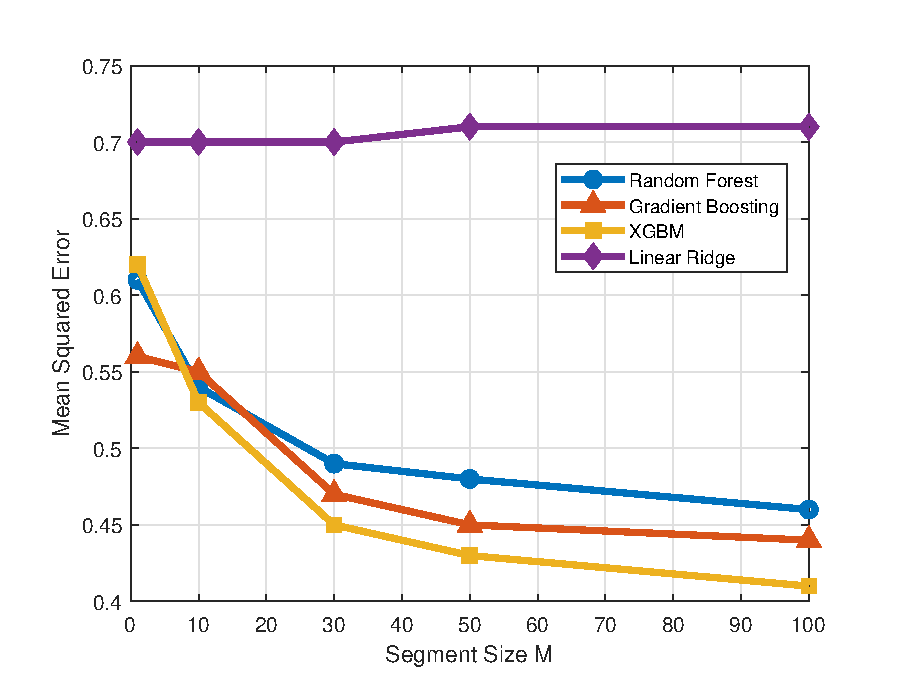
\includegraphics[width=0.75\columnwidth]{./chapter-ftml/plots/001_MSE_M.eps}
	\caption{The mean squared error performance with jamming imposed on b/g-Router of various algorithms against $M$.}
	\label{ftml-jrnl:fig:001_MSE_M}      
\end{figure}

Fig.~\ref{ftml-jrnl:fig:001_R2_M} presents the variance score for the same setting b/g-Router where a similar trend is found. The ensemble-based algorithms can achieves a variance score above 0.35 when $M$ is larger than 50. 

\begin{figure}[!ht]
	\centering
	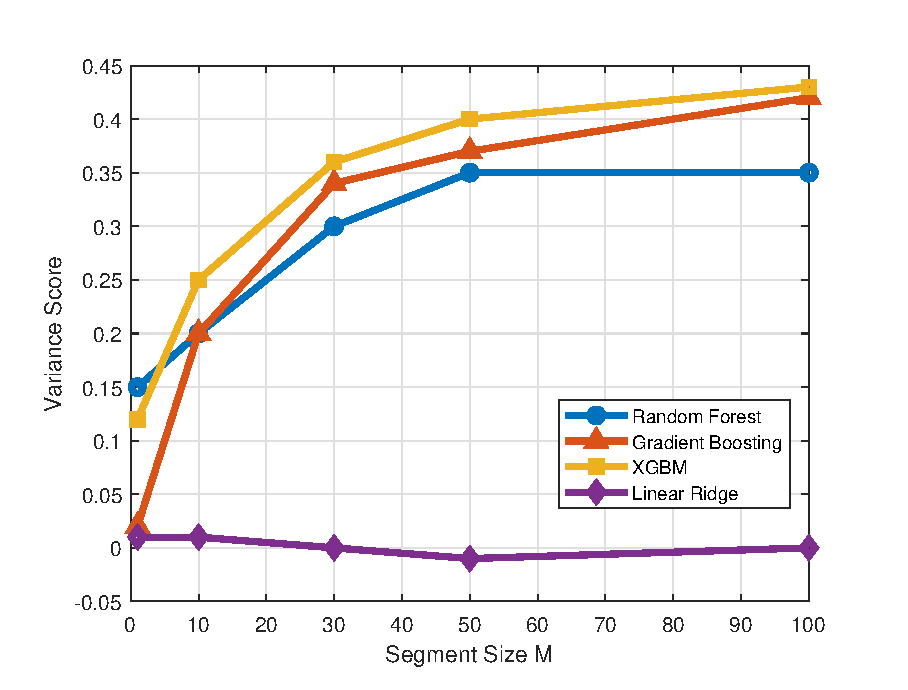
\includegraphics[width=0.75\columnwidth]{./chapter-ftml/plots/001_R2_M.eps}
	\caption{The variance score performance with jamming imposed on b/g-Router of various algorithms against $M$.}
	\label{ftml-jrnl:fig:001_R2_M}      
\end{figure}

In Fig.~\ref{ftml-jrnl:fig:002_MSE_M}, the MSE of the ensemble-based algorithms is shown for Setting b/g-station where the router is impacted by the jamming signal. The MSE values in this setting are lower than those of setting b/g-Router where the predicted SIR values are smaller because the router has better capabilities to detect signals at lower SIRs.    
\begin{figure}[!ht]
	\centering
	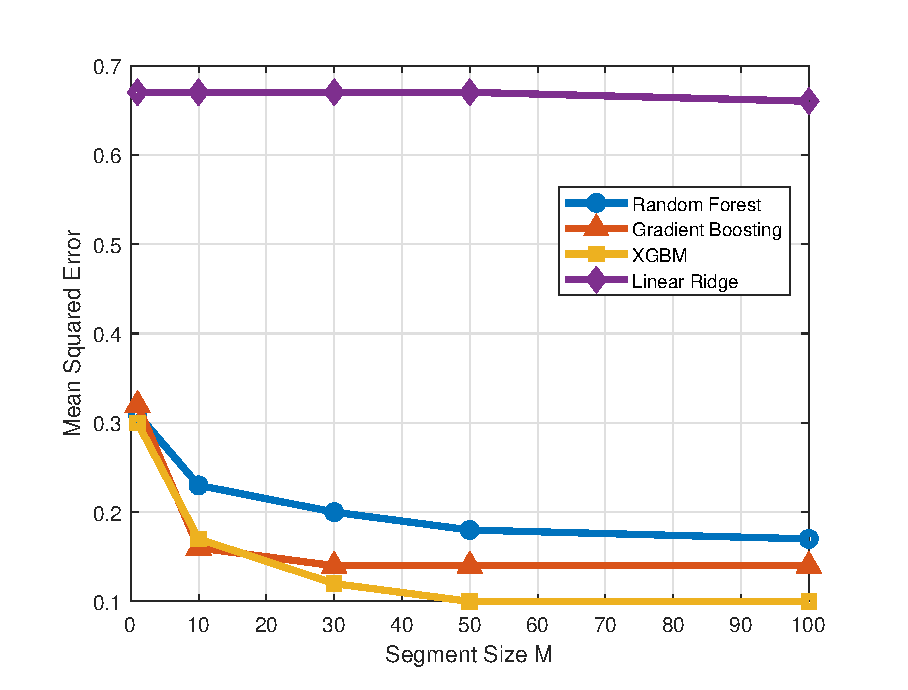
\includegraphics[width=0.75\columnwidth]{./chapter-ftml/plots/002_MSE_M.eps}
	\caption{The mean squared error performance with jamming imposed on b/g-Station of various algorithms against $M$.}
	\label{ftml-jrnl:fig:002_MSE_M}      
\end{figure}

Finally, in Fig.~\ref{ftml-jrnl:fig:004_MSE_M}, a similar scenario to Fig.~\ref{ftml-jrnl:fig:002_MSE_M} is presented where the router is impacted by the jamming signal. The difference is that at setting b/g/n-Station, a mixed IEEE802.11 b/g/n mode is allowed instead the IEEE802.11 b/g mode in setting b/g-Station. By allowing the IEEE 802.11n mode, the signal is more susceptible to interference and hence it is harder to predict the same SIR values. 

\begin{figure}[!ht]
	\centering
	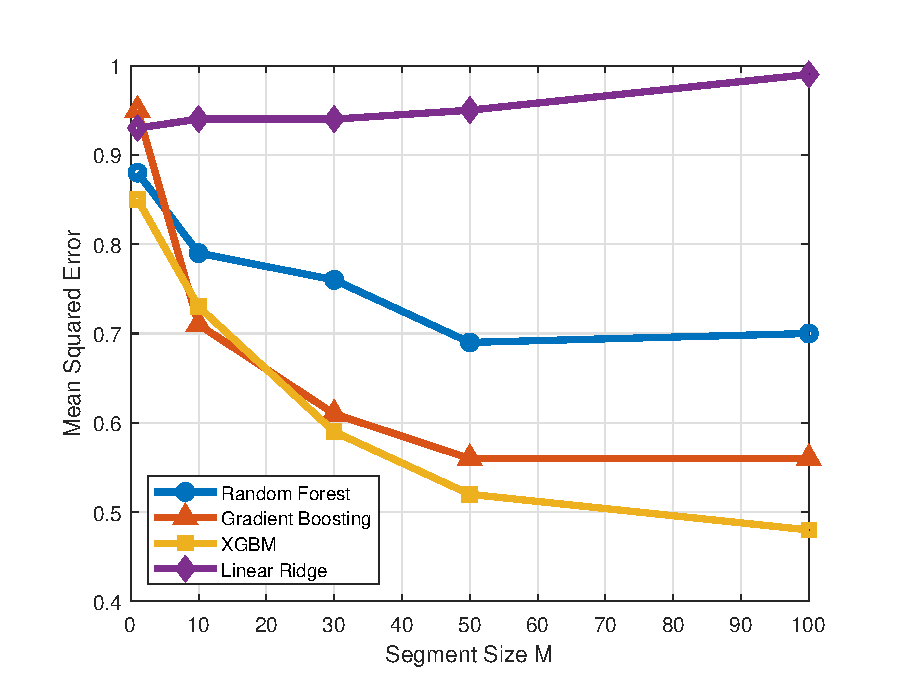
\includegraphics[width=0.75\columnwidth]{./chapter-ftml/plots/004_MSE_M.eps}
	\caption{The mean squared error performance with jamming imposed on b/g/n-Station of various algorithms against $M$.}
	\label{ftml-jrnl:fig:004_MSE_M}      
\end{figure}

\subsubsection{Impact of Training Sequence Length $T$}
This subsection briefly discuss the impact of the training length on the performance of various algorithm. The parameter $T$ is the length of the training sequence where each element contains $M$ of the force seeking cycles. The following figures show the MSE performance curves against $T$ for $M$ = 30 and 100. 

In Fig.~\ref{ftml-jrnl:fig:001_MSE_T}, it is shown that increasing the training size $T$ can improve the prediction performance significantly. Gradient boosting and XGBM have higher improvement rate with $T$ than the random forest algorithm. 
%Moreover, in Fig.~\ref{ftml-jrnl:fig:004_MSE_T}, the random forest is almost not improving at all with $T$ because the prediction algorithm does not perform adequately in this case. 

\begin{figure}[!ht]
	\centering
	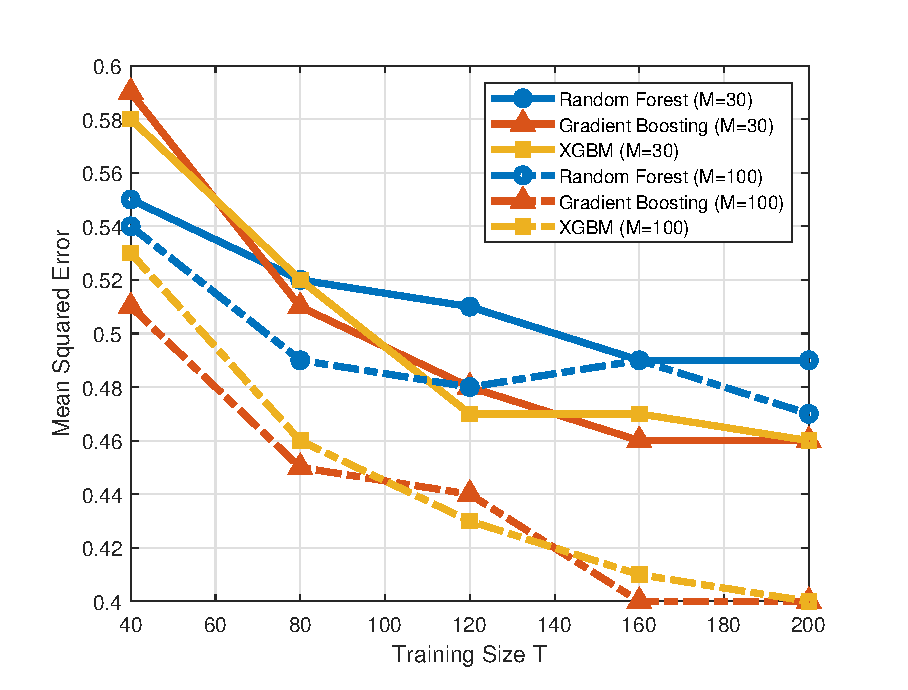
\includegraphics[width=0.75\columnwidth]{./chapter-ftml/plots/001_MSE_T.eps}
	\caption{The mean squared error performance for jamming setting b/g-Router of various algorithms against $T$.}
	\label{ftml-jrnl:fig:001_MSE_T}      
\end{figure}

% 			\begin{figure}[tbp]
% 	    \centering
% 		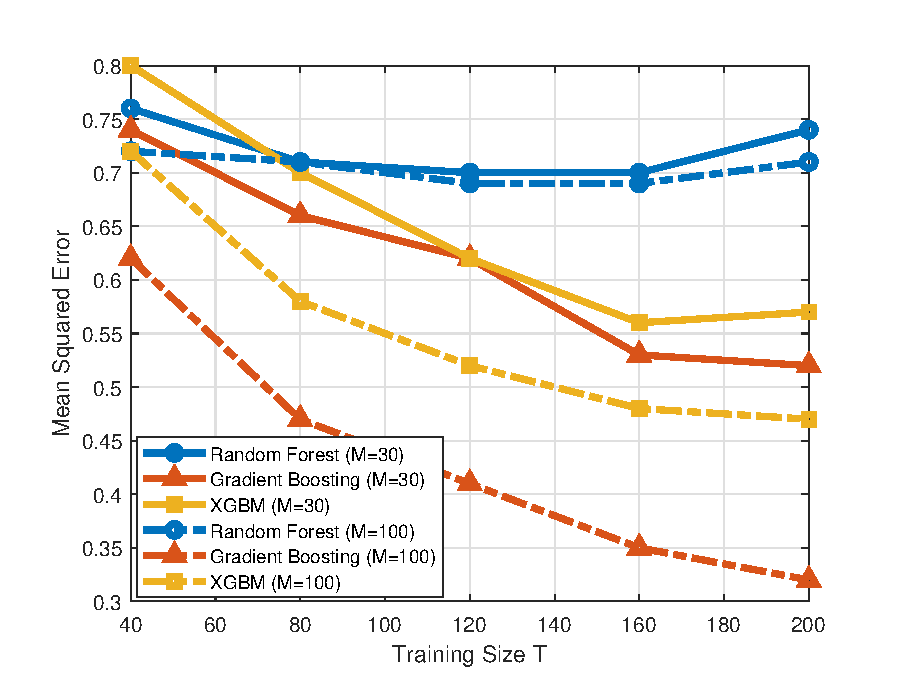
\includegraphics[width=0.8\columnwidth]{plots/004_MSE_T.eps}
% 		\caption{The mean squared error performance for setting 4 of various algorithms against $T$.}
% 		\label{ftml-jrnl:fig:004_MSE_T}      
% 	\end{figure}

\subsubsection{Impact of Individual Features}
In this subsection, the impact of the individual features on the performance of the ensemble-based machine learning algorithms is studied. Understanding the importance of each feature on the prediction algorithms is essential in selection of features and hence reducing the required processing power for an algorithm. The results for XGBM algorithm are shown for brevity and also because it exemplifies the similarity in performance of various ensemble-based algorithms. 

In Fig.~\ref{ftml-jrnl:fig:001_MSE_F_3}, \ref{ftml-jrnl:fig:001_R2_F_3}, and \ref{ftml-jrnl:fig:004_MSE_F_3}, presented are the MSE performance for setting b/g-Router, the variance score for setting b/g-Router, and the MSE for setting b/g/n-Station, respectively, against the segment size $M$. In all the three figures, $\Delta{t}_{ab}$, $\Delta{t}_{bc}$, $Z_d$, $\Delta{t}_{cd}$, and $\Delta{t}_{ae}$ are reference by "t\_high", "t\_plunge", "Descent Distance", "t\_bottom", and "Total Cycle", respectively. 

\begin{figure}[!ht]
	\centering
	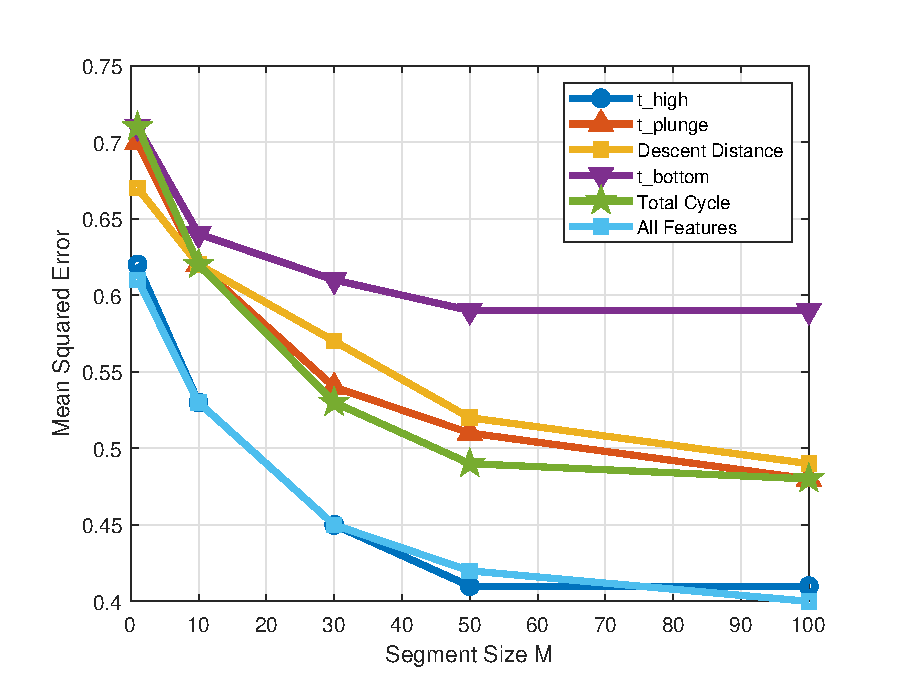
\includegraphics[width=0.75\columnwidth]{./chapter-ftml/plots/001_MSE_F_3.eps}
	\caption{The mean squared error performance for jamming setting b/g-Router of XGBM algorithm against $M$ including individual features impact.}
	\label{ftml-jrnl:fig:001_MSE_F_3}      
\end{figure}

\begin{figure}[!ht]
	\centering
	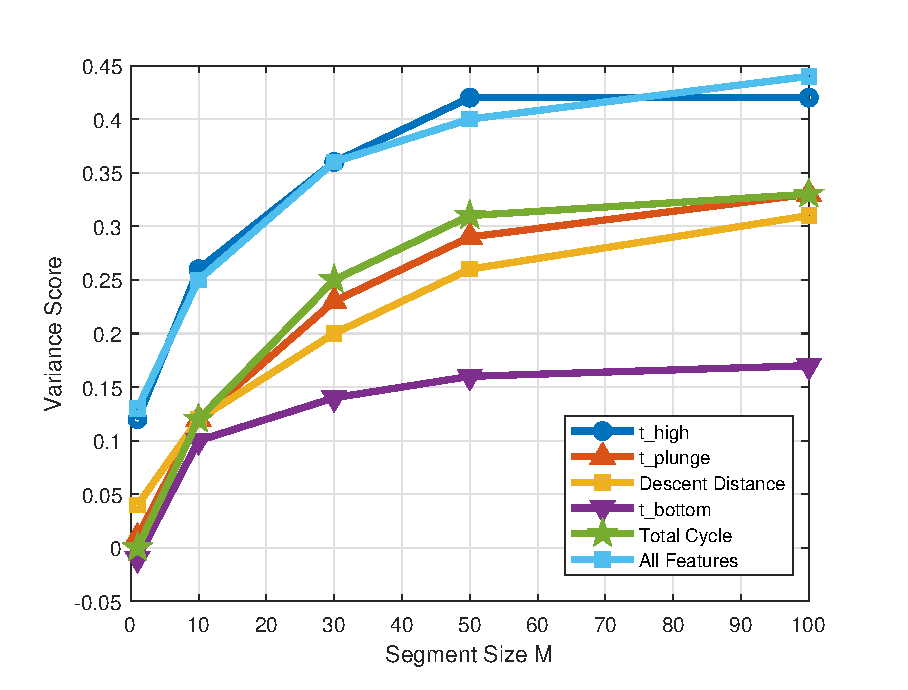
\includegraphics[width=0.75\columnwidth]{./chapter-ftml/plots/001_R2_F_3.eps}
	\caption{The variance score performance for jamming setting b/g-Router of XGBM algorithm against $M$ including individual features impact.}
	\label{ftml-jrnl:fig:001_R2_F_3}      
\end{figure}

\begin{figure}[!ht]
	\centering
	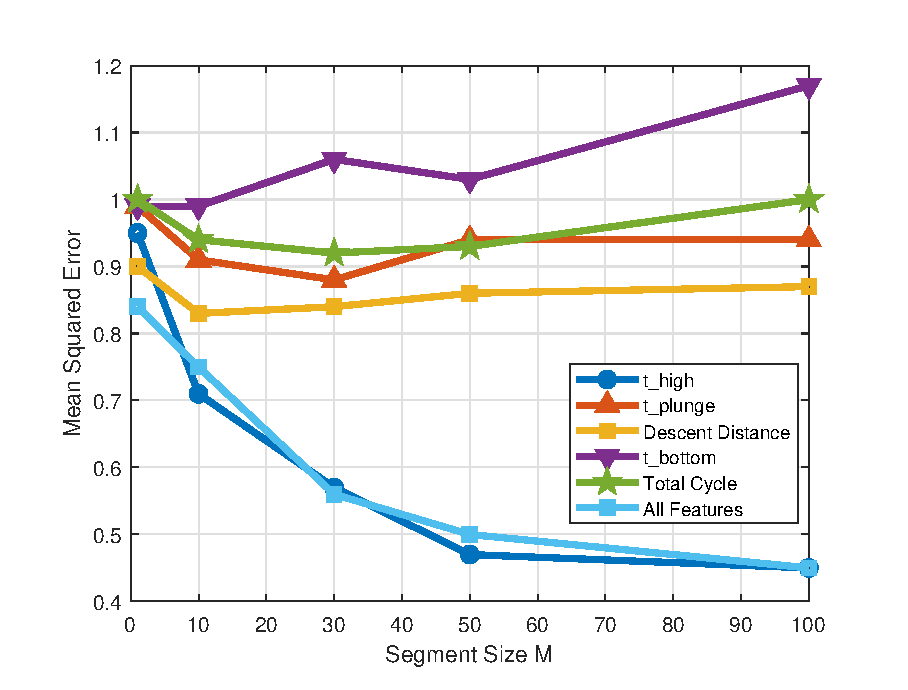
\includegraphics[width=0.75\columnwidth]{./chapter-ftml/plots/004_MSE_F_3.eps}
	\caption{The mean squared error performance for jamming setting b/g/n-Station of XGBM algorithm against $M$ including individual features impact.}
	\label{ftml-jrnl:fig:004_MSE_F_3}      
\end{figure}

The feature $\Delta{t}_{ab}$ is the most one impacted by the SIR value where the prediction performance by using this individual feature is almost identical to the performance of using all the features. This result can be explained by knowing that in the robot arm force seeking program, the FTS has to be zeroed before resuming the loop and hence there is a direct impact of the wireless transmissions and the value $\Delta{t}_{ab}$. On the other hand, the feature $\Delta{t}_{bc}$ is the least one impacted by the SIR value. This feature is defined as the reflection time of the robot arm to reverse its direction and hence it is minimally impacted by the SIR value. The rest of the features are impacted by the SIR to a certain level. Generally, adding an unnecessary feature can degrade the performance. As a result, in this work, it is concluded that using $\Delta{t}_{ab}$ can substitute all the five features to get the same MSE and variance score performance with much less processing.

\begin{emphbox}
	Features selection is a critical step in the application of wireless systems performance analysis with in a cyber-physical system.
\end{emphbox}

\subsection{Conclusion}\label{ftml-jrnl:sec:conclusion}

This work presents a practical use case of a wireless force-torque feedback control system that could be deployed in a manufacturing assembly system such as a pick-and-place or assembly operation.  A 6-DOF force-torque sensor was connected to a robot controller tasked with moving a probe along a linear path until an opposing force exceeding 5 N was detected.  The reliability of the wireless communication system directly impacts the repeatability performance of the physical system are demonstrated.  Also demonstrated was that the quality of the underlying wireless channel may be inferred by observing the position of the probe along a single spatial dimension and applying machine learning to predict the signal-to-interference ratio. As a result of our exploration of various machine learning algorithms on the prediction of signal quality, it was  found that ensemble-based algorithms have superior performance compared to other regression algorithms for data presented.  Additionally, the analysis shows that careful study of the MSE and variance score is useful in selection of features used for training the algorithms. The work concludes that for this particular force-torque control system scenario that the dwell time of the robot before descending was the most useful feature for training the algorithm. The findings provide motivation for applying machine learning to larger more complex systems with higher degrees of freedom. Furthermore, the works indicates that future  experimentation with neural networks and deep learning to improve prediction accuracy could be of value to improving the reliability of wireless operations in factories. The applications of online machine learning techniques to this and other use cases could provide significant benefits to the manufacturing community through integration of link quality detection with programmable controllers.





	
	


